\documentclass[a4paper, 11pt]{book}
\usepackage[utf8]{inputenc}
\usepackage{minted}
\usepackage{graphicx}
\usepackage{hyperref}
\usepackage[linguistics]{forest}
\usepackage{bussproofs}

\usepackage{xpatch}

\makeatletter
\AtBeginEnvironment{minted}{\dontdofcolorbox}
\def\dontdofcolorbox{\renewcommand\fcolorbox[4][]{##4}}
\xpatchcmd{\inputminted}{\minted@fvset}{\minted@fvset\dontdofcolorbox}{}{}
\makeatother

\newenvironment{bprooftree}
  {\leavevmode\hbox\bgroup}
  {\DisplayProof\egroup}
  
\hypersetup{
    colorlinks,
    linkcolor={red!50!black},
    citecolor={blue!50!black},
    urlcolor={blue!80!black}
}
\usepackage[backend=biber,style=alphabetic]{biblatex}
\DeclareUnicodeCharacter{2200}{$\forall$}
\addbibresource{hdr.bib}
\addbibresource{other.bib}

\DeclareSourcemap{
  \maps[datatype=bibtex, overwrite]{
    \map{
      \perdatasource{hdr.bib}
      \step[fieldset=keywords, fieldvalue={, }, appendstrict]
      \step[fieldset=keywords, fieldvalue=me, append]
    }
    \map{
      \perdatasource{other.bib}
      \step[fieldset=keywords, fieldvalue={, }, appendstrict]
      \step[fieldset=keywords, fieldvalue=they, append]
    }
  }
}
%'theorem.py:CoqLexer -x'
\newminted[elpicode]{'elpi.py:ElpiLexer -x'}{fontsize=\small,autogobble,escapeinside=~~,mathescape=true,frame=leftline,framerule=0pt,framesep=1em}
\newminted[elpicodelj]{'elpi.py:ElpiLexer -x'}{fontsize=\small,autogobble,escapeinside=~~,mathescape=true,frame=leftline,framerule=0pt,framesep=0em}
\newmintinline{elpi}{fontsize=\small,autogobble,escapeinside=~~,mathescape=true,frame=leftline,framerule=0pt,framesep=1em}
\newminted[coqcode]{'theorem.py:XCoqLexer -x'}{fontsize=\small,autogobble,escapeinside=~~,mathescape=true,frame=leftline,framerule=0pt,framesep=1em}
\newmintinline{coq}{fontsize=\small,autogobble,escapeinside=~~,mathescape=true,frame=leftline,framerule=0pt,framesep=1em}
 
\newminted[ocamlcode]{'ml.py:OcamlLexer -x'}{fontsize=\small,autogobble,escapeinside=~~,mathescape=true,frame=leftline,framerule=0pt,framesep=1em}
\newmintinline{ocaml}{fontsize=\small,autogobble,escapeinside=~~,mathescape=true,frame=leftline,framerule=0pt,framesep=1em}

\newenvironment{dedication}
  {%\clearpage           % we want a new page          %% I commented this
   \thispagestyle{empty}% no header and footer
   \vspace*{\stretch{1}}% some space at the top
   \itshape             % the text is in italics
   \raggedleft          % flush to the right margin
  }
  {\par % end the paragraph
   \vspace{\stretch{3}} % space at bottom is three times that at the top
   \clearpage           % finish off the page
  }
\title{Elpi: rule-based extension language}
\begin{document}
  
\chapter*{Dedication}
\begin{dedication}
To Cinzia and Anna
\end{dedication}

\setcounter{tocdepth}{5}
\tableofcontents

 \chapter{Introduction}


\section{Prologue}

\subsection{Beyond the odd order theorem}

I had the luck to be part of this project.
After its completion the good question was what it made it possible
other than having Georges Gonthier lead the project. How to make
it possible for others to build such an impressive machine checked
proof. I've always been interested into building tools, since I believe
a tool can democratize...

3 points 1) engineering practices, not new but too often
ignored by the community; 2) formalization technique known as boolean
reflection (or small scale reflection) that carves a light weight
``classical math'' framework in Coq (EM, UIP, FUNEXT) in Coq when
constructivism allows for it; 3) ``creative'' programming of the
Coq elaborator.

We focused on 3. These programs make Coq behave as an informed readers,
that is a reader that knows some base facts and that is expected to
be able to combine them using some well known rules. It was customary,
at that time, to see Coq as a ``dumb reader'': you have to explain
every single detail to him. These programs changed the game  for the
oothm and made it possible to use notations as in math, that is convoy
a lot of information implicitly, by convention.

The objective was to help users craft these programs. Programming
the elaborator as we did was hard. Structuring the library to that
knowledge could be organized by the author an retrieved by these
programs was even harder. The programming mechanism is called CS,
and is strictly related to the UH I studied during my PhD.
Independently, about at the same time,
Coq got extended with type classes, which happened to be usd for similar
purposes, and immediately raised similar programming issues.

To my eyes, these programs were strikingly related to Prolog.
Our programs were organized in rules and driven by unification.
At that time I had barely heard about Prolog.
It happened that the Parsifal team
at Inria Saclay worked on a language or that family
and thanks to Assia Mahboubi and Stephane Legrand I could give a talk
at a STTT workshop they were hosting.

In my talk I did explain some of the programs we wrote and why they
were helping us writing math in Coq. Dale Miller, asked a few questions
and suggested that his $\lambda$Prolog language was probably what I
was looking for, but since I did not know anything about it I could
just nod and ask to continue to the discussion offline.

not just the rules but also their animation and maybe also the entire
elab algorithm.

Dale was kind
to set up a meeting with Claudio Sacerdoti and myself. 

\subsection{The beginning: a snowy day}

On that day ``Paris'' was frozen, in the sense that a supposedly
``show storm'' convinced authorities to close buildings and other facilities,
reduce public transportations to the bare minimum. For some reasons
the XXX building was not closed, so the 3 of us agreed to buy a sandwich,
walk up the hill (with boots) and meet in a desert building.

After two hours of gentle introduction, after having savoured the
elegance of \elpiinline{copy}, I clearly remember I say ``sold...'',
but I also completed the sentence with ``how do I do evars?''.

$\lambda$Prolog could easily describe the rules my programs were
made of and elegantly manipulate the data type of Coq terms that
notably contains many binders. But also holes, evars in Coq slang,
that are the other beast one has to tame in order to implement an
elaborator and, in general, the outern layers of a toll like Coq.

It was the beginning.

Teyjus in bologna, we could write a toy elaborator in one day
but we could not find a good solution. Reification is ugly, one has
to pass a subst and reimplement unif. At the same time reusing unif
variables seemed possible, but extremely hard since the pure core
of LP, and Teyjus, do not really give you systems to control their
assignment and an elaborator takes in input a term with holes
and returns a term where only some holes are assigned...

It was worth trying but using teyjus in Matita or Coq was too hard.
I write a POC interpreter of LP in OCaml for embedding it into
Matita and Coq, elpi. It was easy to add hacks and experiment with
it, and that ... Elab in matita was kind of working, we could run
it on the arithmetic library. It was clear that:
the perf were bad, very bad, like 22K times bad.
the hacks could be explained in terms of constraints and rules to
suspend, resume, combined them.


\section{Elpi}
Elpi is both a language and an implementation of that language.

With CSC we rewrote the runtime, first the FO part then the HO part
and 

line stats

I perceived many times, in academic circles, some mistrust in logic programming.


We organize this document in four parts. The first two describe Elpi from
A to Z, both as a language and as an implementation of that language (we credit
\cite{ridoux1998lambda}). The third describes the integration of Elpi in Coq
and the fourth one surveys the application developed for Coq using Elpi.


\chapter{Elpi the language: \emph{de A \`a Z}}

Elpi is a mix of two languages: $\lambda$Prolog and Contraint Handling Rules.
The former is a higher order variant of Prolog based on
Hereditary Harrop Formulas, a generalization of Horn Clauses.
The latter is language to manipulate a store of constraints that,
in the case of Elpi, is made of suspended goals, i.e. sequents
made of heigenvariables, dynamic rules and a conjecture.

We briefly introduce all the ingredients that constitute Elpi.
Most of the syntax of Elpi is inherited from $\lambda$Prolog, as well
as the type discipline~\cite{Miller_Nadathur_2012}; similarly most of
its dynamic semantics is inherited from Prolog.
We state this upfront with no claim of novelty and but we just say Elpi in what
follows. We shall still highlight the novelties or simply differences from
$\lambda$Prolog or Prolog as they appear.

\section{Elpi v.s. Prolog}

Regarding an introduction to Prolog, the reader is spoiled for choice.
Here, we limit ourselves to establishing the terminology and highlighting
the key characteristics of Elpi and differences from standard Prolog from the
perspective of the programmer. We identify three of them: data types, rules
and search.

The first feature worth pointing out is algebraic data types, such as
list and trees. Here the declaration of binary tress in Elpi syntax:

\begin{elpicode}
kind tree type.
type leaf tree.
type node int -> tree -> tree -> tree. 
\end{elpicode}

The \elpiinline{leaf} and \elpiinline{node} function symbols can be used to
build ``compound terms'' and have arity 0 and 3 respectively. Elpi
follows the tradition of typed functional languages by prescribing not only
an arity but a more precise type to \elpiinline{leaf} and \elpiinline{node}.
In this document we refer to them as term constructors, or simply constructors.
Types play no role at run time but grately contribute to the static analysis
of the code, allowing to report typos and sometime even true errors early.

Here an example of the three

\begin{forest}
  [46 [93 [-] [-]] [-]]
\end{forest}

\begin{elpicode}
T = (tree 46 (tree 93 leaf leaf) leaf)
\end{elpicode}
  
To the reader familiar with
Prolog we point out that Elpi adopts the syntactic convention
of $\lambda$-calculus for function calls, namely $(f~ x~ y)$ rather than the
mathematical convention $f(x,y)$ adopted by Prolog.

The second feature we discuss is that the code is organized into
rules, that constitue the smallest code unit\footnote{In this document we prefer the
word rule to clause.}. A rule is made of two parts, the head and the premises.
Intuitively the head drives the selection of a rule, reducing the current
problem, that we goal, to simpler ones. Operationally the head is unified with the
goal, possibly assigning value to the rule parameters that are embodied by
unification variables. For example code computing the size of a tree, together
with its signature:

\begin{elpicode}
type size tree -> int -> prop.
size leaf 0.
size (node _ L R) N :- size L N1, size R N2, N is 1 + N1 + N2.
\end{elpicode}

Again we favor a type assignment to a simple arity. \elpiinline{prop} is the
type of executable code, meaning that \elpiinline{size}, when applied to two
arguments, becomes a goal and a program can be run to solve it.
On the contrary \elpiinline{node}, applied to any number of arguments,
is just a piece of data, it is not a goal.

\begin{elpicode}
goal> size T N.

Success
  N = 2
\end{elpicode}

Operations on built-in data types, such as integers, are provided via
the built-in \elpiinline{is} operator that evaluates its right hand side
and unifies the result with the left hand side.

It is worth pointing out that variables do not need to be used linearly
in the head of a rule: since the head is unified with the goal, it makes sense to
write there any therm, not just terms that happen to be patterns in
the sense of functional programming languages. For example the following
piece of code succeeds only if the tree is empty or made of two
identical subtrees.

\begin{elpicode}
type symmetric tree -> prop.
symmetric leaf.
symmetric (node _ T T).
\end{elpicode}

The third characteristic is that Elpi internalizes a form of search called
backtracking: all rules are potentially applied and there is no committment to
the first rule whose head unifies with the goal.
Here an example of code relying on backtracking to test
the membership of an element ot a tree.

\begin{elpicode}
type mem tree -> int -> prop.
mem (node N _ _) N.
mem (node _ L _) N :- mem L N.
mem (node _ _ R) N :- mem R N.
\end{elpicode}

Backtracking is a very powerful feature but without control leads to
unnecessarily bad computational complexity. The one contruct to control
backtracking is the cut operator.

\begin{elpicode}
mem (node N _ _) N :- !.
mem (node _ L _) N :- mem L N, !.
mem (node _ _ R) N :- mem R N.
\end{elpicode}  

Operationally the cut is not a premise to be solved, but rather telling
the runtime the intention to commit to the current rule and solution.
The former cut indicates that if the number is found in the current node
we commit to this rule and discard the following ones: we do not care
if the number also occurs deeped in the tree. The second cut indicates
that if the number was found in the left sub tree we shall not look in
the right sub tree so we discard the last rule\footnote{To be precise
the second cut also discard any alternative solution (yet to be computed)
to the preceeding premises. Technically speaking, Elpi implements a hard cut.}.

\subsection{What really matters (to us)}

Algebraic data types are an essential tool to write succint code
to describe and process syntax trees. They are available in languages
from the Prolog family, but also in most functional languages. Hence they do
not constitute the feature that tips the balance in favor of a logic
programming language.

On the contrary functional languages do not usually come with backtracking
while it is undeniable that logic programming and backtracking are linked by
a strong bond and that the ability to ``compute relations'' is a typical
selling point. Still, according to our experience, the vast majority of code
written in Elpi does not need this feature.

So, in conclusion, I believe that the most interesting
characteristic of logic programming is of being a rule based language.

It trades the elaborate syntax offered by most
programming languages with the notion of a smaller code unit.
A code unit has a meaning per se and the operation of adding or removing it
to/from a program is well defined.

An assignment, a while loop, or a function definition do not
constitute a code unit. An assignment is meaningless without a variable
declaration, similarly a while loop: they only get a meaning, even a formal 
one, in a larger context. Even the definition of a self contained function fails to be a unit in
this sense: while adding it to a program makes some sense (although, since nobody
calls it, serves little purpose),
removing a used function just results in a non functional program.

A rule has a meaning given by its logical interpretation. Adding it or removing
it from a logic program simply results in a different logic program. Typically
by adding a rule the resulting program is able to handle one more case,
a bit like a proof system lets you prove more statements if one poses
more axioms, or becomes more and more incomplete as axioms are removed.
From the parallel with proof systems it is obvious that adding ``bad'' rules
can result in a program that gives unexpected answers, but the operation
of adding or removing them is still meaningful, even if one admits non logical
constructs and departs for the ideal world of logic.
If we admit non logical
constructs then the order of rules becomes relevant and the insertion of a
rule better be accompanied by a grafting directive, like begin added before
or after another rule.

It it thanks to this rule-based nature that logic programming scales so
naturally to the domain of syntax trees with binders (next section)
and that it integrates so well with interactive provers (see~\ref{sec:rocq}).

\section{Elpi v.s. $\lambda$Prolog}

The syntax trees we are interested in are the ones that constitute
the foundational language of interactive provers like Coq. A characteristic common
to all of the them is the presence of binders, as forall and exists in
the world of specification or (lambda) abstraction in the world of terms.

The ``hello world'' example in this domain is simply typed lambda calculus,
a formalism now almost a century old. The syntax of terms and types
is declared as follows:

\begin{elpicode}
kind term type.
type lam (term -> term) -> term.
type app term -> term -> term.

kind ty.
type arr ty -> ty -> ty.
\end{elpicode}

The type declaration for terms introduces a pairing constructor \elpiinline{app},
putting together a function and its argument, and a function former
\elpiinline{lam} that abstracts a term over a (bound) variable representing the
formal argument. The declaration uses the function space of
the programming language in order to represent the abstraction:
the function carried by \elpiinline{lam} can be applied to an actual argument in order
to recoved the body of the expression where the formal argument is
replaced by the actual argument.

In this syntax the fst function is written as follows:

\begin{elpicode}
Fst = (lam x\ lam y\ x)
\end{elpicode}

Note that \elpiinline{(x\ lam y\ x)} is a function of \elpiinline{x} (a
variable of the Elpi programming language)
and that the syntax tree of our object language, $\lambda$-calculus, does not
feature a term constructor for variables since one can reuse the variables
of Elpi.
As sketched above the body of the first abstraction
can be recovered by applying the function: \elpiinline{((x\ lam y\ x) c)}
gives \elpiinline{(lam y\ c)}.


% \begin{elpicode}
% type copy term -> term -> prop.
% copy (lam F) (lam G) :- pi x\ copy x x => copy (F x) (G x).
% copy (app A B) (app C D) :- copy A C, copy B D.
% \end{elpicode}

The type checker for the simply typed $\lambda$-calculus can be implemented by
the following two rules:

\begin{elpicode}
type of term -> ty -> prop.
of (app H A) T :- of H (arr S T), of A S.
of (lam F) (arr S T) :- pi c\ of c S => of (F c) T.
\end{elpicode}

The rule for application reads: in order to assign type \elpiinline{T} to
the application of \elpiinline{H} to \elpiinline{A} we need to assign
the type \elpiinline{S} arrow \elpiinline{T} to \elpiinline{H} and
the type \elpiinline{S} to \elpiinline{A}. The one for abstraction
assigns the type \elpiinline{S} arrow \elpiinline{T} if, given any
fresh symbol \elpiinline{c} of type \elpiinline{S} the body of
the function \elpiinline{F} has type \elpiinline{T} when the bound variable
is substituted by \elpiinline{c}.


The two rules above closely match the ``inference rules'' commonly used in
by the logic or programming language communities:
\label{inf:stlc}

$$
\begin{bprooftree}
  \AxiomC{$\Gamma \vdash e_1 : \sigma \to \tau$}
  \AxiomC{$\Gamma \vdash e_2 : \sigma$}
  \BinaryInfC{$\Gamma \vdash e_1~e_2 : \tau$}
\end{bprooftree}
\qquad
\begin{bprooftree}
  \AxiomC{$\Gamma, c : \sigma \vdash e[x/c] : \tau \quad c~\mathrm{fresh~in}~\Gamma$}
  \UnaryInfC{$\Gamma \vdash \lambda x.e : \sigma \to \tau$}
\end{bprooftree}
$$



The main difference is that $\Gamma$ is managed by Elpi: the \elpiinline{pi}
operator guarantees the freshness of $c$, while \elpiinline{=>} augments
the current program with an instance of the rule:

$$
\begin{bprooftree}
  \AxiomC{$x : T \in \Gamma$}
  \UnaryInfC{$\Gamma \vdash x : T$}
\end{bprooftree}
$$

While Prolog finds it roots on Horn clauses, $\lambda$Prolog and hence
Elpi are based on Hereditary Harrop formulas~\cite{}. While the rule for application
can be seen as a formula in the Horn fragment:

$$
\mathrm{of}~ H~(\mathrm{arr}~S~T) \land \mathrm{of}~A~S \Rightarrow \mathrm{of}~(\mathrm{app}~H~A)~T
$$

\noindent the rule for lambd aabstraction truly needs the $\forall$ quantifier
and the use of (nested) implication:

$$
(\forall c, \mathrm{of}~c~S \Rightarrow  \mathrm{of}~(F~c)~T) \Rightarrow \mathrm{of}~(\mathrm{lam}~F)~(\mathrm{arr}~S~T)
$$

The reading of the rule for abstraction as an Hereditary Harrop formula
makes it clear that the scope of $c$ and the so called hypothetical rule
assigning it a type are limited to the subgoal $\mathrm{of}~(F~c)~T$,
unlike the \texttt{assert/1} and \texttt{retract/1} Prolog builtins\footnote{
  although some Prolog implementation provide the notion of ``transation''
that can be used to simulate scoping.}.

As previously announced, we want to use Elpi in the contet of an
interactive prover like Coq where syntax trees are often incomplete, i.e.
they contain holes. For example we would like to run the
type checker of this goal: \elpiinline{of (app F A) T}.

This is where $\lambda$Prolog falls short, by lack of a way to avoid
divergence by suspending search on certain goals and lack of a sub language
to manipulate suspended goals.


\subsection{Incomplete terms}

$\lambda$Prolog provides native support for syntax trees with bound
variables via the re-use of the function space of the programming language
to represent binders. This technique is called Higher Order Abstract Syntax,
or $\lambda$-tree syntax. The language also provides another kind
of variables, meta-variables actually, that we call unification variables.
These unification variables are equipped with a scope, a list of bound
variables that can be used in their assignment. This is essential to
avoid capturing variables by mistake, and it is well studiend in~\ref{}.

The natural question is: can we reuse the unification variables of
the programming language to represent holes in the syntax trees we manipulate?
In other words, the runtime of of our Logic programming language is already
carrying a substitution for these variables, undoing its application upon
backtracking, avoiding the generation of circular terms (i.e. not trees)
by performing occur check, and avoiding captures: can we reuse all that?

Elpi tries to give a positive answer to this question. Moreover it provides
support to attach data to holes ``on the side'', similarly to what
hypothetical rules are used for in the type checker above: attach a type
to fresh constants.

From a programming perspective, the needs are the following ones:

\begin{description}
  \item[control instantiation of holes] in particular be able to opt out of the
     generative behavior of Prolog based on the order of rules. According to
     our experience when a hole is encountered one of the following two
     actions need to be implemented: either suspend the computation and
     generate a constraint, or synthesize an assignment for the hole
     via a dedicated routine
  \item[attach data to holes] from a simple boolean flag, as we will do
    when implemeting ML type inference with equality types,
    to a full typing sequence as it is necessary to do when holes represent
    Coq terms

  \item[manipualte attached data] such as combine multiple data attached to the same
     hole or perform a consistency check when the hole gets assigned

\end{description}


\section{Modes and Constraints}\label{sec:modes}

Elpi provides a notion of mode declaration that is uncommon to logic programming.
In particular arguments that are flagged as input are not required to be
ground in the goal, but are matched against the rule ``pattern'' instead 
of being unified. This means that no unification variable occurring in
the goal inside an input argument is instantiated when the rule is
fired.

Mode declaration comes together with the \elpiinline{uvar} keyword to denote
holes in the head of a rule.

In the light of that we can rephrase the type checker for simply typed $\lambda$-calculus
as follows:

\begin{elpicode}
pred of i:term, o:ty.
of (app H A) T :- of H (arr S T), of A S.
of (lam F) (arr S T) :- pi c\ of c S => of (F c) T.
of (uvar as E) T :- declare_constraint (of E T) [E].
\end{elpicode} 

The \elpiinline{pred} directive combines a type and mode declaration.
The \elpiinline{uvar as E} binds to the unification variable \elpiinline{E}
a hole in the goal and is semantically equivalent to the following,
where \elpiinline{var/1} is the standard Prolog predicate testing if
a variable is unbound.
  
\begin{elpicode}
of E T :- var E, declare_constraint (of E T) [E].
\end{elpicode}

Many Prolog implementations feature a ``delay directive'' sublanguage to
prescribe when goals should be suspended or resumed. In Elpi we opeted for
a more low level but also more flexible approach where the programmer declares
constraints / suspends goal via  the \elpiinline{declare_constraint} built-in
predicate. In the example above \elpiinline{[E]} is the list of variables
that ``block'' the suspended goal: as soon as one is assigned the goal should
be resumed.

It is worth pointing out that the input mode described above can in principle
we ``emulated'' via a program transformation that we sketch below:

\begin{elpicode}
of E T :- not (var E), E = (app H A), of H (arr S T), of A S.
of E (arr S T) :- not (var E), E = (lam F), pi c\ (of E S :- not (var E), E = c) => of (F c) T.
of E T :- var E, declare_constraint (of E T) [E].
\end{elpicode}

With this mechanism in place the type checker can do something useful
on terms containing holes:

\begin{elpicode}
goal> of (app H A) T.
Success:

Constraints:
  of A S  /* suspended on A */
  of H (arr S T)  /* suspended on H */
\end{elpicode}

The resumption 

\begin{elpicode}
goal> of (app H A) T, H = (lam x\ x).

Success:

Constraints:
  of A T  /* suspended on A */
\end{elpicode}

And the very same result is given on the goal \elpiinline{of (app (lam x\ x) A) T}.
  
Unfortunately the sole possibility of suspending and resuming goals is
not enough to implement a satisfactory type checker. An example of
goal giving an unexpected result is \elpiinline{of (app D D) T}
that succeeds with constraints

\begin{elpicode}
  of D S  /* suspended on D */
  of D (arr S T)  /* suspended on D */
\end{elpicode}

that are clearly incompatible.

We need a language to combine the constraints attached to hole \elpiinline{D}.

\section{Constraints Handling Rules}

A C.H.R.~\cite{chr}
program is a set of rules that maintain the constraint store, a
multi-set of (suspended) goals. A rule adds or removes constraints
from the store, and rules are applied following their order
as per the refined operational semantics~\cite{10.1007/978-3-540-27775-0_7}
of C.H.R.

The following Elpi code complements the running example by
imposing that each hole has only one typing constraint.

\begin{elpicode}
constraint of {
  rule (of X T1) \ (of X T2) <=> (T1 = T2)
}
\end{elpicode}

The rule reads: if the constraint \elpiinline{of X T1} is present
in the store together with \elpiinline{of X T2}, then remove
the latter and generate a new goal \elpiinline{T1 = T2}.
This is sufficient to make the type checker
reject \elpiinline{of (app D D) T}, since the goal
\elpiinline{S = arr S T} fails (because of occur check).

A detail to remak is that the constraints are matched against
the constraint handling rules, that is the non linear occurrence
of \elpiinline{X} does not risk to ``merge'' two unrelated constraints:
the rule above only applied if two constraint about the same variable
are in the stote.

Another important difference is that constraint handling rules
match more goals at once. While the execution of an Elpi program
can be seen as a depth-first construction of a proof tree, with
the possibility of suspending the exploration of a branch, the
application of a constraint handling rule operates on all suspended
branches. In a way it is a ``meta'' proof search step. It can for
example identify to identical subgoals and share/connect their (missing)
proof. Indeed CHR rules do have a logical reading.

\begin{verbatim}
rule G1 \ G2 | T <=> G3
\end{verbatim}

This rule is sound if, somehow, if $T \land G1 \Rightarrow (G2 \Leftrightarrow G3)$
  
As we mentioned before Elpi automatically manages the context, that is
the set of fresh constants generated by \elpiinline{pi} and hypothetical
rules introduced by \elpiinline{=>}. As a result an Elpi goal is
not just a predicate $P$, but rather a sequent $E \triangleright  \Gamma \vdash P$
where $E$ is the set of fresh constants and $\Gamma$ the set of hypothetical rules.

The previous rule to model uniqueness of typing is hence incomplete
since the same hole can occur under different contexts. This more
elaborate version accepts different contexts and sets of fresh constants.

TODO explain S1 S2 \cite{joijgov}.

\begin{elpicode}
constraint of {
  rule (E1 :> G1 ?- of (uvar X S1) T1) \ (E2 :> G2 ?- of (uvar X S1) T2)
    <=> (T1 = T2)
}
\end{elpicode}

While correct for simple types this rule does not scale for a type
discipline like the one of Coq where terms can occur in types,
i.e. where the constants in S1 occur in T1, and S2 in T2. In this
richer setting comparing T1 and T2 in the disjoint union is incorrect,
one needs to relocate one term under the context of the other in order
to unify them (and avoid pruning, TODO example)

bla $E1 \uplus E2 \triangleright \emptyset \vdash G$ where $\uplus$.

The most precise constraint handling rule is the following one:

\begin{elpicode}
constraint of {
  rule (E1 :> G1 ?- of (uvar X S1) T1) \ (E2 :> G2 ?- of (uvar X S1) T2)
    | (relocate L1 L2 G1 G2 T2 T2')
    <=> (E1 :> G1 => T1 = T2)
}
\end{elpicode}

First, \elpiinline{uvar X S} is the syntax for the unification variable X
with scope S, where S is a list of constants. The guard of the rule $G$,
namely \elpiinline{relocate L1 L2 G1 G2 T2 T2'}, runs as a Elpi goal
$E1 \uplus E2 \triangleright \emptyset \vdash G$ where $\uplus$ denotes

TODO: Example of abs evars?

Constraints and CHR serve many purposes:
\begin{itemize}
  \item justify/implement some non-logical operations
  \item implement a state and its management
  \item schedule constraints
\end{itemize}

\section{Elpi = $\lambda$Prolog + CHR}\label{sec:elpiLP+CHR}

Elpi integrates the SLD search strategy typical of Prolog with
CHR as depicted:

%\begin{figure}
  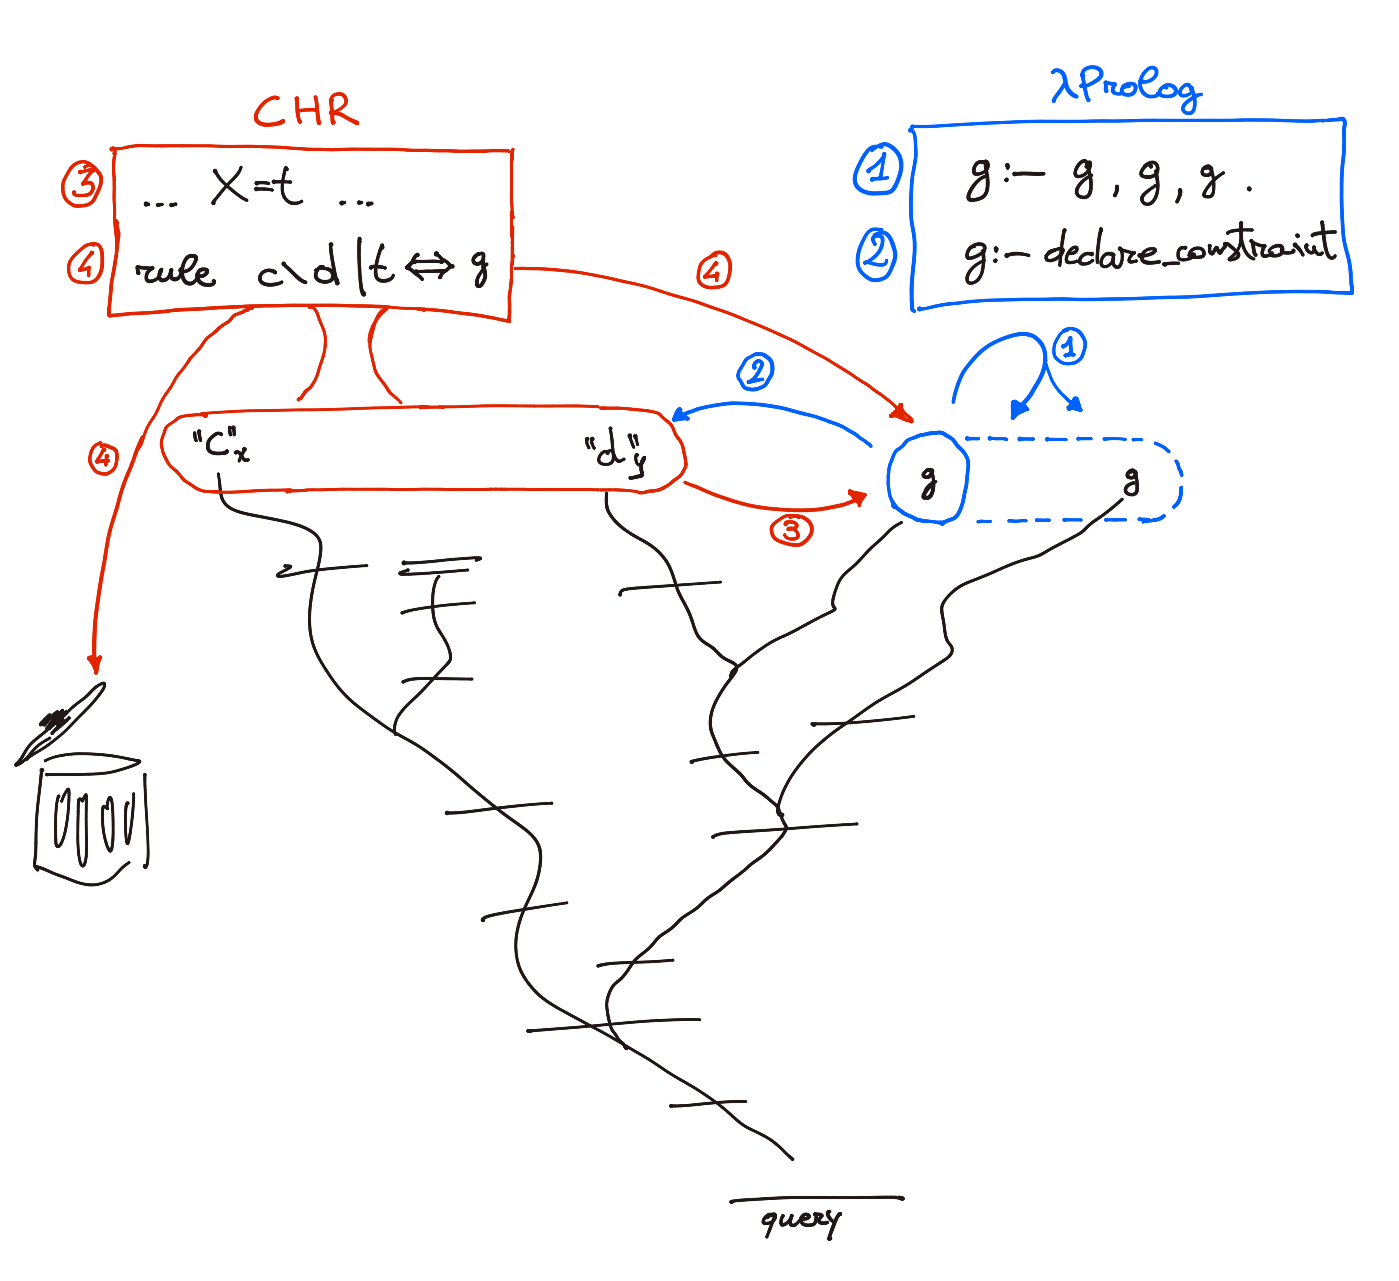
\includegraphics[width=0.8\textwidth]{chr.png}
%  \caption{\label{chr:fig}Elpi runtime (TODO clause/rule)}
%\end{figure}



 
Rule application follows the refined operational semantics~\cite{10.1007/978-3-540-27775-0_7}.
It amounts to precise neting of iterations. The starting point is
the so called ``active constraint'' $A$ that, in the context of Elpi, is
the constraint just declared via \elpiinline{declare_constraint}.

\begin{enumerate}
\item for each rule $P_1 \ldots P_x \backslash P_{x+1} \ldots P_n | C \Leftarrow G$
\item for each position $0 < j \leq n$
\item for each permutation of $C_1 \ldots C_n$ constraints having $C_j = A$
\item match all $C_i$ with $P_i$ and run $C$. If it succeeds:
  \begin{itemize}
    \item remove $C_{x+1} \ldots C_n$ from $\mathcal{C}$
    \item remove all permutations involving $C_{x+1} \ldots C_n$
  \end{itemize}
\item move to the next rule
\end{enumerate}

The semantics described above, most of the times, behaves intuitively: rules
are scanned in order and applied when applicable. It becomes a bit surprising,
accorsing to our experience, when the multiset nature of the constraint store
plays a role, in particular when permutations contain duplicate predicates.


\begin{center}\begin{minipage}{.6\textwidth}
%elpi:chr.elpi
\begin{elpicodelj}
pred c i:int.

main :-
  print "declare c 1",
  declare_constraint (c 1) [_],
  print "declare c 2",
  declare_constraint (c 2) [_].
\end{elpicodelj}
\end{minipage}
~\\
\vspace{1em}
~\\
\bgroup
\setlength{\tabcolsep}{1em}
\begin{tabular}{c c}
\begin{minipage}{.44\textwidth}
%elpi:chr1.elpi
\begin{elpicodelj}
constraint c {
  rule (c N) (c M) <=>
    (print "rule 1 on" N M).
  rule (c N) <=>
    (print "rule 2 on" N).
}
\end{elpicodelj}
\end{minipage} &
\begin{minipage}{.44\textwidth}
%elpi:chr2.elpi
\begin{elpicodelj}
constraint c {
  rule (c N) \ (c M) <=>
    (print "rule 1 on" N M).
  rule (c N) <=>
    (print "rule 2 on" N).
}
\end{elpicodelj}
\end{minipage} \\
\\
\vspace{1em}
\begin{minipage}{.44\textwidth}
\begin{verbatim}
declare c 1
rule 2 on 1
declare c 2
rule 1 on 2 1
rule 1 on 1 2
rule 2 on 2
\end{verbatim}
\end{minipage} &
\begin{minipage}{.44\textwidth}
\begin{verbatim}
declare c 1
rule 2 on 1
declare c 2
rule 1 on 2 1

rule 2 on 2
\end{verbatim}
\end{minipage}
\end{tabular}
\egroup
\end{center}
~\\

According to the rule set on the left hand side of the figure,
rule 1 triggers twice since the second \elpiinline{c} constraint
is active in both position 1 and 2. This is also the case
in the second rule set, but since the rule remove one (copy) of
\elpiinline{c} from the store and hence from the permutations set,
the rule cannot trigger twice.

Integration with SLD works as follows: each new constraint becomes
a goal that is considered as the leftmost conjuct of the current
resolution state. Since a new goal can in turn declare a new constraint,
the CHR loop can continue. In other words constraint handling takes
priority over SLD resolution.

\section{Syntactic sugar}

Elpi features some simple syntactic sugar that is elimated by
the ``compiler'' before running programs.

\subsection{Namespaces}

Elpi code is obtained by accumulating together files, that is
``concatenating'' lists of rules, possibly written by different
authors. It is not impossible that
two files, file1 and file2, contain declarations for a predicate with same name p.

When the types for p do not match, Elpi fails immediately
and the programmer is warned. But when the types match, it may
happen that the predicate changes meaning or complexity,
especially in case of failure.

A simple man solution could be to simply put the file name
as part of predicate names, eg file1.p and file2.p.

To paliate the syntactic overhead Elpi provides two syntactic
facilities: namespace and shorten. The former prefixes all
names of the predicates contained in a block, the latter makes
predicates accessible via a short name inside a file or a block

\begin{elpicode}
namespace n1 {
  pred p.
}
\end{elpicode}

elsewhere

\begin{elpicode}
shorten n1.{ p }.
q :- p.
\end{elpicode}

note that a type/mode declaration declares the belonging to a namespace.

\begin{elpicode}
p.
namespace n2 {
  pred p.
  q :- p.
}
\end{elpicode}

\subsection{Spilling}

We argue that the names we give to the objects we manipulate
are the most important form of documentation and badly chosen
name are the primary cause of unreadable code.

The time a sloppy programmer saves by using \elpiinline{TMP}, \elpiinline{AUX}
or \elpiinline{X'} instead of thinking at an appropriate name is
demanded, with interests, to any reader of code, including himself.

Logic programming, even in its Higher Order flavor, distinguishes
commands from expressions (predicates from data). This characteristic
is the primary contributor to the proliferation of temporary
variables, a phenomenon that functional programming languages
reduce by putting in the same syntactic category function calls an
data. 

For example the OCaml code \texttt{List.rev (List.append l1 l2)}
or its equivalent \texttt{List.append l1 l2 |> List.rev} enables
to programmer to avoid naming the result of append, while in logic
programming one often reads

\begin{elpicode}
code L1 L2 Result :- append L1 L2 TMP, rev TMP Result.
\end{elpicode}

Elpi provides a syntatic facility to let one use
``partially applied'' predicates as ``function calls''.
By partially applied we mean ``applied to all the arguments flagged as input''.
For example the code above can be written as follows

\begin{elpicode}
code L1 L2 Result :- rev {append L1 L2} Result.
\end{elpicode}

The curly braces identify a term to be \emph{spilled} to the closest
\emph{execution point}, identified by walking the terms outside in and
identifying the first expression of type \elpiinline{prop}.

Spilling can be nested. Its elaboration is akin to the generation
of the administrative normal form that is commonly used in functional
programming languages.

\subsubsection{Spilling under a binder}

When the spilled expression needs to cross a binder in order to
reach the execution point, the elaboration is more sophisticated.
For example: 

\begin{elpicode}
code Result :- Result = (lam x\ {mk-app f [x]}).
code Result :- (pi y\ mk-app f [y] (TMP y)), Result = (lam x\ TMP x).
\end{elpicode}
  

In order to run the spilled code in a context with the bound variable
x, the expression must be put under a \elpiinline{pi y\\ }. Similarly
the temporary variable needs to be abstracted over the variable, so
that we can identify the original one x with the one abstracted by
\elpiinline{pi} y.

Note that spilling does not need to cross a \elpiinline{pi}, but
needs to make the quantified variable visible to the result of
the spilled computation, for example explicilty quantifying it
with a sigma. For example:

\begin{elpicode}
  code L1 L2 Result :- pi x\ rev {append [x|L1] L2} (Result x).
  code L1 L2 Result :- pi x\ sigma TMP\ append [x|L1] L2 TMP, rev TMP (Result x).
\end{elpicode}

\subsubsection{Spilling and impliction}

When the object language features a sophisticated HOAS for the context
(as in \ref{GALLINA}) it may be necessary to augment the context with
the implication operator. For example imagine the \elpiinline{lam}
term constructor carries the type of the bound variable

\begin{elpicode}
  code Ty Result :- Result = (lam Ty x\ lam {of x Ty => of (app g x)} y\ ...)
  code Ty Result :-
    (pi x\ of x Ty => of (app g x) (TMP x))
    Result = (lam Ty x\ lam (TMP x) y\ ...)
\end{elpicode}

This is frequent when spilling combined with quotations, for example

\begin{elpicode}
  T = {{ fun x : nat => lp:{{ app f {api x}  }}  }}
\end{elpicode}

where the api needs the context of the object language, see \ref{FFI}

\paragraph{Spilling ambiguities}

Not all that glitter is gold. Sometimes the closest execution
point may not be what the programmer wants.

\begin{elpicode}
  code D TodoForLater  :-
    TodoForLater [ this, that {rev D} ].
\end{elpicode}

If this and that are predicated, the latter becomes
\elpiinline{(rev D TMP, that TMP)} meaning that
D is reversed when TodoForLater will be executed, and
not when the todo list is generated, as one may have wanted.

According to our experience the closes execution point
is more often than not what the programmer expects.

\section{A complete example: Hindley Milner type inference}

The most significan type inference algorith is the one crafted by
Milner the ML language~\cite{MILNER1978348}. The flavor we 
study here covers equality type variables, the \texttt{''a} abstraction
(in standard ML syntax) for decidable types, i.e. types that can be
effectively compared unlike the function space.

It makes a good use case for Elpi because:
\begin{itemize}
  \item it manipulates syntax trees with binders, namely lambd abstraction
    and let binding
  \item it manipulates types containing unification variables (i.e. holes).
    The key step in the algorithm is to turn (existentially quantified)
    unification variables into universally quantifies type variables to
    form a skema
  \item unification variables have an attribute, a flag (denoted with
    an over bar) that is set if the equality test is used on values
    of their type.
\end{itemize}

The syntax of terms is very similar to the simply typed $\lambda$-calculus
one, with the addition of \texttt{let} and the equality test. We omit
conditional, loops or recursion since it does not play an important role.

\begin{center}
\begin{minipage}{0.35\textwidth}
$$
\begin{array}{lrl}
  e & =     & x                                 \\
  & \vert & e_1\ e_2                            \\
  & \vert & \lambda\ x\ .\ e                    \\
  & \vert & \mathtt{let}\ x = e_1\ \mathtt{in}\ e_2 \\
  & \vert & e_1 = e_2 \\
\end{array}
$$
\end{minipage}
\begin{minipage}{0.55\textwidth}
\vspace{0.5em}
%elpi:hm.elpi
\begin{elpicodelj}
kind term type.
type global  string -> term.
type app term -> term -> term.
type lam (term -> term) -> term.
type let term -> (term -> term) -> term.
type eq  term -> term -> term.
\end{elpicodelj}
\end{minipage}
\end{center}
~\\  
~\\  
As in section~\ref{} we use an HOAS encoding of terms.
Still we add a \elpiinline{global} term constructor to
be able to set up a minimal environment for our examples.

Monomorphic type expressions $\tau$ and type skemas $\sigma$
are depicted below. As in the original paper we fix a few builtin type contructors
instead of supporting a generic n-ary type former, but unlike
the ML tradition we put type constractors to the left of an application.
We use the infix symbol \elpiinline{-->} for the function space of ML.

\begin{center}
\begin{minipage}{0.4\textwidth}
$$
\begin{array}{lrl}
  \\
    \tau   &=     & \alpha                    \\
                              &\vert &  \tau \to \tau         \\
                              &\vert &  \mathtt{int}         \\
                              &\vert &  \mathtt{bool}         \\
                              &\vert &  \mathtt{list}\ \tau         \\
                              &\vert &  \mathtt{pair}\ \tau\ \tau         \\
  
     \sigma &=    & \tau                                           \\
                             &\vert& \forall\ \alpha\ .\ \sigma \\
                            &\vert& \forall\ \bar\alpha\ .\ \sigma \\
  \\
\end{array}
$$
\end{minipage}
\begin{minipage}{0.5\textwidth}
%elpi:hm.elpi
\begin{elpicodelj}
kind tye type.
type (-->) tye -> tye -> tye.  
type int   tye.
type bool  tye.
type list  tye -> tye.
type pair  tye -> tye -> tye.

kind ty type.
type all    bool -> (tye -> ty) -> ty.
type mono   tye -> ty.
\end{elpicodelj}
\end{minipage}
\end{center}


The typing routing works with a context and, as we did for the
simply typed lambda calculus, we delegate its management to the
programming language.

$$
\begin{array}{llrl}
  \\
    \text{Context}     & \Gamma & = & \epsilon\ \mathtt{(empty)}\\
                       &        & \vert& \Gamma,\ x : \sigma\\
    \text{Typing}      &        & = & \Gamma \vdash e : \sigma\\
  \\
  \end{array}
$$


We give below a fre example of type assignement to global
constants. It is worth highlighting the fact that the
type skema for \elpiinline{"undup"}


%elpi:hm.elpi
\begin{elpicode}
pred of i:term, o:ty.
of (global "1")      (mono int).
of (global "plus")   (mono (int --> int --> int)).
of (global "nil")    (all ff x\ mono (list x)).
of (global "cons")   (all ff x\ mono (x --> list x --> list x)).
of (global "pr")     (all ff x\ all ff y\ mono (x --> y --> (pair x y))).
of (global "fst")    (all ff x\ all ff y\ mono (pair x y --> x)).
of (global "size")   (all ff x\ mono (list x --> int)).
of (global "undup")  (all tt x\ mono (list x --> list x)).
\end{elpicode}
  

The specialization of type skema allows one to plug type expressions in place
of quantified variables. When the substituted variables stands for an
equality type, one has to check that the type expression has an equality test.

$$
\displaystyle\frac{\tau' = \left\{\alpha_i \mapsto \tau_i\right\} \tau \quad \beta_i \not\in \textrm{free}(\forall \alpha_1...\forall\alpha_n . \tau)}{\forall \alpha_1...\forall\alpha_n . \tau \sqsubseteq \forall \beta_1...\forall\beta_m . \tau'}
$$
$$
\displaystyle\frac{\tau' = \left\{\bar\alpha_i \mapsto \tau_i\right\} \tau \quad \beta_i \not\in \textrm{free}(\forall \alpha_1...\forall\alpha_n . \tau) \quad \overline{eq}(\tau_i)}{\forall \alpha_1...\forall\alpha_n . \tau \sqsubseteq \forall \beta_1...\forall\beta_m . \tau'}
$$
$$
\begin{array}{ll}
  \overline{eq}(\mbox{bool}) & \\
  \overline{eq}(\mbox{int}) & \\
  \overline{eq}(\mbox{list}~\tau) & ~\mbox{if}~ \overline{eq}(\tau) \\
  \overline{eq}(\mbox{pair}~\tau_1~\tau_2) & ~\mbox{if}~ \overline{eq}(\tau_1) ~\mbox{and}~ \overline{eq}(\tau_2)\\
  \overline{eq}(\bar\alpha) & \\
\end{array}
$$

The Elpi code departs the pen and paper presentation by instantiatin, at once,
all skema variables by fresh unification variables, possibly constraining them
to be an eq type

%elpi:hm.elpi
\begin{elpicode}
pred specialize i:ty, o:tye.
specialize (mono T) T.
specialize (all ff F) T :- specialize (F Fresh_) T.
specialize (all tt F) T :- specialize (F Fresh) T, eqbar Fresh.
\end{elpicode}

The \elpiinline{eqbar} predicate traevrses concrete type expressions and
suspend when variables are found.

%elpi:hm.elpi
\begin{elpicode}
pred eqbar i:tye.
eqbar bool.
eqbar int.
eqbar (list A) :- eqbar A.
eqbar (pair A B) :- eqbar A, eqbar B.
eqbar (uvar as A) :- declare_constraint (eqbar A) [A,_].

constraint of ?- gammabar eqbar theta rm-eqbar {
  rule (eqbar V) \ (theta L) | (not(mem L V)) <=> (theta [V | L]).
}

pred theta i:list tye.
theta L :- declare_constraint (theta L) [_].
\end{elpicode}

The auxiliary constraint \elpiinline{theta} is used to gather the
(duplicate free) list of unification variables constrained to be equality types.

The use of constraints here is handy but not essential. One could thread a state,
the list of all type variables used so far paired with their equality type status.
The constraint store offers a global state carried on the side of the goals
and constraint handling rules the possibility to organize it, like grouping
all entries into a list.

The declarative code for the type inference algorithm is given below.
While the rules for lambda abstraction and application are the same
for simply typed lambda calculus~\ref{inf:stlc}.

\begin{center}
\begin{minipage}{0.45\textwidth}
$$
\begin{array}{cl}
  \displaystyle\frac{\Gamma \vdash e_0:\tau \rightarrow \tau' \quad\quad \Gamma \vdash e_1 : \tau }{\Gamma \vdash e_0\ e_1 : \tau'}\\ \\
  \displaystyle\frac{\Gamma,\;x:\tau\vdash e:\tau'}{\Gamma \vdash \lambda x.e : \tau \rightarrow \tau'}
\end{array}
  $$
\end{minipage}
\begin{minipage}{0.45\textwidth}
$$
\begin{array}{cl}
  \displaystyle\frac{x:\sigma \in \Gamma \quad \sigma \sqsubseteq \tau}{\Gamma \vdash x:\tau}\\ \\
  \displaystyle\frac{\Gamma \vdash e_0:\tau \quad\quad \Gamma,\,x:\bar{\Gamma}(\tau) \vdash e_1:\tau'}{\Gamma \vdash \mathtt{let}\ x = e_0\ \mathtt{in}\ e_1 :  \tau'}
  \end{array}
$$
\end{minipage}
$$ 
\displaystyle\frac{\Gamma \vdash e_1 : \tau \quad \Gamma \vdash e_2 : \tau \quad \overline{eq}(\tau)}{\Gamma \vdash e_1 = e_2: \mathtt{bool}}
$$
\end{center}

The rule for variables finds in $\Gamma$ a skema and assigns to the variable
any valid instance. The rule for let pushes into the context a type
$\overline{\Gamma}(\tau)$ for a let-bound expression of type $\tau$ in $\Gamma$.
Finally the rule for equality tests if the type of the expressions admits
an equality test.

%elpi:hm.elpi
\begin{elpicode}
of (app H A) (mono T) :-
  of H (mono (S --> T)),
  of A (mono S).

of (lam F) (mono (S --> T)) :-
  pi x\ of x (mono S) => of (F x) (mono T).

of (let E B) (mono TB) :-
  of E (mono T),
  gammabar (mono T) PT,
  pi x\ of x PT => of (B x) (mono TB).

of (eq LHS RHS) (mono bool) :-
  of LHS (mono T),
  of RHS (mono T),
  eqbar T.

of X (mono T) :- of X (all E Poly), specialize (all E Poly) T.
\end{elpicode}

Elpi rules are very close to pen and paper ones. The only difference is that
the rule for variable is extended, on purpose, to any term so that it
can apply to global constants as well.

We have already described how \elpiinline{specialize} relates to $\sqsubseteq$,
what is left to describe is the $\overline{\Gamma}$ operation.
  
$$
\overline{\Gamma}(\tau) = \forall\ \hat{\alpha}\ .\ \tau \quad\quad \hat{\alpha} = \textrm{free}(\tau) - \textrm{free}(\Gamma)
$$

Intuitively one has to compute the free type variables in $\Gamma$ and $\tau$
and only abstract the ones as not free in $\Gamma$, i.e. that are only used
locally to the expressions being bound by the let.

This operation escapes the capabilities of $\lambda$Prolog alone, even with
the mode extensions we discuss in~\ref{sec:modes}, since $\Gamma$ is not
first class or in other words it is automatically managed by the runtime.
This is where the ``meta'' status of constraint handling rules comes in
handy: suspended goals are sequents made of a formula and its context.

%elpi:hm.elpi
\begin{elpicode}
pred gammabar i:ty, o:ty.
gammabar (mono T) TS :- declare_constraint (gammabar (mono T) TS) [_].

constraint of ?- gammabar eqbar theta rm-eqbar {
  rule  \ (theta L)
          (G ?- gammabar T TS)     % matched and removed
        | (generalize L G T POLYT ToRemove) % guard + syntesis
      <=> (TS = POLYT, rm-eqbars ToRemove, theta []).             % new goal
  rule \ (eqbar X) (rm-eqbar X).
}

pred rm-eqbars i:list tye.
rm-eqbars [].
rm-eqbars [X|XS] :- rm-eqbar X, rm-eqbars XS.

pred rm-eqbar i:tye.
rm-eqbar X :- declare_constraint (rm-eqbar X) [X, _].

pred generalize i:list tye, i:list prop, i:ty, o:ty, o:list tye.
generalize Theta Gamma (mono T) PolyT ToQuantify :-
  free-ty (mono T) [] VT,
  free-gamma Gamma [] VGamma,
  filter VT (x\ not(mem VGamma x)) ToQuantify,
  bind ToQuantify Theta T PolyT.
\end{elpicode}

The code to implement $\overline{\Gamma}(\tau)$ performs thwo tasks:

\begin{itemize}
  \item It abstracts \elpiinline{T} into a skema \elpiinline{POLYT} and
    returns is by assigning \elpiinline{TS}
  \item It cleans up the store of constraints removing the \elpiinline{eqbar}
    constraints on variables that are now bound in the skema, and updates
    \elpiinline{theta} by recomputing it
\end{itemize}

The first task is necessary while the second one is mainly to explain an motivate
the scheduling choices described in~\ref{sec:elpiLP+CHR}. In particular it is crucial
that all unneeded \elpiinline{eqbar} constraints are removed before
\elpiinline{theta} is recomputed by combining the new constraint with all
\elpiinline{eqbar} constraints still in the store. It is also worth notion how
the (declarative) semantics of CHR grants that the new \elpiinline{theta}
constraints is combined with all \elpiinline{eqbar} ones, no matter in
which order they are added to the store: up to now \elpiinline{theta} was
there and was updated at every \elpiinline{eqbar} addition; now all
\elpiinline{eqbar} are there, and \elpiinline{theta} gets added and combined
with the all.

The code for computing free type variables is as expected.

$$
\begin{array}{ll}
  \text{free}(\ \mathtt{int}\ ) &=\ \emptyset\\
  \text{free}(\ \mathtt{bool}\ ) &=\ \emptyset\\
  \text{free}(\ \mathtt{pair}\ \tau_1\ \tau_2\ ) &=\ \text{free}(\ \tau_1\ )\cup \text{free}(\ \tau_2\ ) \\
  \text{free}(\ \mathtt{list}\ \tau\ ) &=\ \text{free}(\ \tau ) \\
  \text{free}(\ \tau_1 \to \tau_2\ ) &=\ \text{free}(\ \tau_1\ )\cup \text{free}(\ \tau_2\ ) \\
  \text{free}(\ \alpha\ ) &=\ \left\{\alpha\right\}\\
  \text{free}(\ \forall\ \alpha\ .\ \sigma\ ) &=\ \text{free}(\ \sigma\ )\  -\  \left\{\alpha\right\}\\
  \text{free}(\ \Gamma\ ) &=\ \bigcup\limits_{x:\sigma \in \Gamma}\text{free}(\ \sigma\ )\\
\end{array}
$$

Two details of the corresponding Elpi code are worth pointing out.

The former is that the context is a list of propositions. The \elpiinline{prop}
type gather all predicates, not just \elpiinline{of}. We don't need to add
a rule skip any unrelated predicate the program may have loaded with implication
because the \elpiinline{constraint of ?- gammabar eqbar theta rm-eqbar} directive
tells Elpi to filter the context of suspended goals (constraint) and keep only
entries for the \elpiinline{of} predicate.

The second is that, at the meta level of constraint handling rules, the
\elpiinline{uvar} keyword becomes a regular syntax tree node and that is
has two arguments. The first one is the unique identifier of the unification
variable. The second one is its scope represented as a list of names.
  

%elpi:hm.elpi
\begin{elpicode}
pred free-ty i:ty, i:list tye, o:list tye.
free-ty (mono X) L L1 :- free X L L1.
free-ty (all _ F) L L1 :- pi x\ free-ty (F x) L L1.

pred free-gamma i:list prop, i:list tye, o:list tye.
free-gamma [] L L.
free-gamma [of _ T|X] L L2 :- free-ty T L L1, free-gamma X L1 L2.

pred free i:tye, i:list tye, o:list tye.
free int L L.
free bool L L.
free (list A) L L1 :- free A L L1.
free (pair A B) L L1 :- free B {free A L} L1.
free (A --> B) L L1 :- free B {free A L} L1.
free (uvar _ _ as X) L L1 :- if (mem L X) (L1 = L) (L1 = [X|L]).
\end{elpicode}

The last bit of code necessary to implement $\overline{\Gamma}(\tau)$ is
the code to bind (locally used) unification variables to universal quantifications.
The key is the \elpiinline{copy} predicate~\cite{}, that reflects substitution
by traversing a type expression. Since this subtitution is not the built-in
one (i.e. not function application), we can alter its behavior by loading
into the program context some ad-hoc rules. In particular for
each variable \elpiinline{uvar X _} to abstract we postulate a fresh symbol
\elpiinline{c} and we load a rule to copy \elpiinline{uvar X _} to \elpiinline{c}.

%elpi:hm.elpi
\begin{elpicode}
pred bind i:list tye, i:list tye, i:tye, o:ty.
bind [uvar X _|XS] Theta T (all E x\ T1 x) :- % load the substitution
  if (mem Theta (uvar X _)) (E = tt) (E = ff),
  pi c\ (copy (uvar X _) c :- !) => bind XS Theta T (T1 c).
bind [] _ T (mono T1) :- copy T T1. % fire the substitution

pred copy i:tye, o:tye.
copy int int.
copy bool bool.
copy (list A) (list B) :- copy A B.
copy (pair A B) (pair C D) :- copy A C, copy B D.
copy (A --> B) (C --> D) :- copy A C, copy B D.
copy (uvar _ _ as V) V.
\end{elpicode}

For completeness the remaining code follows. It may be worth explaining the
signature of the polymorphic, higher order, \elpiinline{filter} predicate.
In particular \texttt{i:(pred i:A)} stands for an input predicate over
\elpiinline{A}, where the predicate itself expects an input.

%elpi:hm.elpi
\begin{elpicode}
pred mem i:list tye, i:tye.
mem [uvar X _|_] (uvar X _) :- !.
mem [_|XS] X :- mem XS X.
 
pred filter i:list A, i:(pred i:A), o:list A.
filter [] _ [].
filter [X|XS] F [X|YS] :- F X, !, filter XS F YS.
filter [_|XS] F YS :- filter XS F YS.
\end{elpicode}

The code amounts to about 100 lines of Elpi. It is a toy, in the sense
that its lacks code for error reporting, but its size is quite remarkable:
it roughly mathes the length of a pen and paper presentation of the same
algorithm.

\subsection{A word on bidirectionality}

Maybe the most unexpected feature of the running example is that
it is a bidirectional algorithm. In particular the rule for application
pushed dowh the expected type of the argument when type checking it.

The mono-directional version could look like the following code:

\begin{elpicode}
of (app H A) (mono T) :-
  of H (mono TH),
  of A (mono TA),
  assert H TH (TA --> T).

pred assert i:term, i:tye, i:tye.
assert _ TY ETY :- TY = ETY, !.
assert T TY ETY :-
  halt "Error: term" T "has type" TY "but its context expects" ETY.
\end{elpicode}

Note how \elpiinline{TH} is not related to \elpiinline{TA} before the
call to  \elpiinline{of A (mono TA)}, and how the code only checkes
after the facts that \elpiinline{TH = (TA --> T)}.

\section{Pitfalls}

During these years we gave Elpi in the hands of a
good number of users. Here the pitfalls that tricked everybody (ourself included).

\subsection{Misleading precedence of \elpiinline{=>}}

When one write \elpiinline{A, B => C, D} means
\elpiinline{A, B => (C, D)}. This is clear when
one has a program \elpiinline{A, B => D} and wants
to sneak in a print to debug before D.

So we argue that \elpiinline{=>} should bind stronger than ,
on the left but not on the right, something parsing
technology does not support out of the box. We introduced
\elpiinline{==>} that parses with these precedences and add a warning
whenever \elpiinline{A, B => C, D} that can be silenced
by writing \elpiinline{A, (B => C), D}.

\subsection{Treacherous anonymous clauses}

HO lets one write \elpiinline{map L (x\r\p x A, q A r) L'}
where A is quantified (allocated) in the wrong place.
The correct way is \elpiinline{map L (x\r\sigma A\p x A, q A r) L'},
but we believe it would be way safer to only allow (partially
applied) predicates as HO arguments.

The syntactic overhead is often compensated by the extra
reading clarity a (well) named predicate provides.

\subsection{Scope error as a (recondite) failure}

While \elpiinline{pi x\ F = x} clearly fails because x is
out of scope, its practical, legit, use cases are rare.
Most of the times when a unification fails because of
a scope problem, it is dues to a user mistake.

Although we have not tried to implement any measure to help
newcomers, we wonder if making this cause of unification failure
fatal (as is aborting the program) would help newcomers quickly
identify the true mistake.

%%%%%%%%%%%%%%%%%%%%%%%%%%%%%%%%%%%%%%%%%%%%%%%%%%%%%%%%%%%%%%%%%%%%%55
%%%%%%%%%%%%%%%%%%%%%%%%%%%%%%%%%%%%%%%%%%%%%%%%%%%%%%%%%%%%%%%%%%%%%55
%%%%%%%%%%%%%%%%%%%%%%%%%%%%%%%%%%%%%%%%%%%%%%%%%%%%%%%%%%%%%%%%%%%%%55
%%%%%%%%%%%%%%%%%%%%%%%%%%%%%%%%%%%%%%%%%%%%%%%%%%%%%%%%%%%%%%%%%%%%%55

\chapter{Elpi the software: \emph{de A \`a Z}}

\section{The first prototype}

The first Elpi was written by Tassi in about 3 months, with the objective
of understanding the $\lambda$Prolog language and some of the techniques
adopted to implement it, like the suspension calculus~\cite{NADATHUR200235}.
This was Elpi-POC

Terms were purely functional, to ease backtracking. This feature comes
with a reputation of making things hard, so we played conservative.

Suspension calculus did look similar to exp-substitutions, but until the very
last last paper in the pile on my desk it was not clear is was actually isomorphic
to $\lambda_\rho$. While explicit substitutions are often presented as a way to
obtain better performances, in practice they fail to deliver. In Coq two
people tried. In elpi-POC, in our limited tests, disabling them resulted in
a faster runtime.  bla bla about lazyness.

Elpi-POC was an easy playground to understand which features were needed in
order to manipulate terms with holes: a safeguard against instantiating them by
mistake (modes) and a was to attach metadata to holes (constraints).

Elpi-POC was functional enough to let us write an elaborator for CIC
and plug it into Matita. It was working, but it was too slow. Line 20K times
slower than reasonable.

Reason number one was the purely functional heap, with no GC. Introducing 
instructions to clear memory (in an unsafe way) was enough to see order of
magnitude fade.

\section{Second attempt: a runtime for $L_{\lambda}^{\beta}$}

imperative terms with a trail did not cause bugs, but a sensible speedup.
DBL made HO code sensibly faster \cite{dunchev15lpar}.

\subsection{The $L_{\lambda}$ fragment}
\subsection{The $L_{\lambda}^{\beta}$ fragment}

\cite{Michaylov1993HigherOrderLP}

built in lists.

CHR is still naive.

The compiler performs very little optimizations. In recent years its speed
in extending existing programs became relevant, since state is encoded as rules.

\subsection{Indexing}
\subsubsection{Patricial tree (over bits)}

predicate to index
symbol to clauses

special bucket for flex arg or flex input arg

\subsubsection{Hash map}

multiple arg, variable depth. similar perf


\section{The API}

The APIs to drive the interpreter essentially lets one parse code, comile into
unit, assemble units and run it.

In addition to that and FFI and quotations

\subsection{Quotations}

the one rule is that a variable is bound in one language and only
one.

example from the tutorial

\begin{elpicode}
  coq.say {{ 1 + lp:{{ app[global S, {{ 0 }} ]  }}   }}
% elpi....  coq..     elpi...........  coq  elpi  coq
\end{elpicode}


\subsection{FFI}\label{FFI}

FFI is akin to printf, given a first class description of
the types of the arguments it performs the conversion
back and forth.

The peculiarity is that the context and constraint store
is given too to the conversion functions. In particular
this enables a tight integration see \ref{GALLINA}.

the FFI makes extensive use of GADTs.

contextual conversion

\begin{ocamlcode}
module Conversion : sig

type 'a embedding =
  depth:int ->
  Data.state -> 'a -> Data.state * Data.term * extra_goals

type 'a readback =
  depth:int ->
  Data.state -> Data.term -> Data.state * 'a * extra_goals

type 'a t = {
  ...
  pp : Format.formatter -> 'a -> unit;
  embed : 'a embedding;   (* 'a -> term *)
  readback : 'a readback; (* term -> 'a *)
}
\end{ocamlcode}


\begin{ocamlcode}
module ContextualConversion : sig

type ('a,'hyps,'constraints) embedding =
  depth:int -> 'hyps -> 'constraints ->
  Data.state -> 'a -> Data.state * Data.term * Conversion.extra_goals

type ('a,'hyps,'constraints) readback =
  depth:int -> 'hyps -> 'constraints ->
  Data.state -> Data.term -> Data.state * 'a * Conversion.extra_goals

type ('a,'h,'c) t = {
  ...
  pp : Format.formatter -> 'a -> unit;
  embed : ('a,'h,'c) embedding;   (* 'a -> term *)
  readback : ('a,'h,'c) readback; (* term -> 'a *)
}

type ('hyps,'constraints) ctx_readback =
  depth:int -> Data.hyps -> Data.constraints ->
  Data.state -> Data.state * 'hyps * 'constraints * Conversion.extra_goals
\end{ocamlcode}


\begin{ocamlcode}
module BuiltInPredicate : sig

type ('function_type, 'inernal_outtype_in, 'internal_hyps, 'internal_constraints) ffi =
  (* Arguemnts that are translated independently of the program context *)
  | In    : 't Conversion.t * doc * ('i, 'o,'h,'c) ffi -> ('t -> 'i,'o,'h,'c) ffi
  | Out   : 't Conversion.t * doc * ('i, 'o * 't option,'h,'c) ffi -> ('t oarg -> 'i,'o,'h,'c) ffi

  (* Arguemnts that are translated looking at the program context *)
  | CIn    : ('t,'h,'c) ContextualConversion.t * doc * ('i, 'o,'h,'c) ffi -> ('t -> 'i,'o,'h,'c) ffi
  | COut   : ('t,'h,'c) ContextualConversion.t * doc * ('i, 'o * 't option,'h,'c) ffi -> ('t oarg -> 'i,'o,'h,'c) ffi

  (* The easy case: all arguments are context independent *)
  | Easy : doc -> (depth:int -> 'o, 'o, unit, unit) ffi

  (* The advanced case: arguments are context dependent, here we provide the
    context readback function *)
  | Full : ('h,'c) ContextualConversion.ctx_readback * doc -> (depth:int -> 'h -> 'c -> Data.state -> Data.state * 'o * Conversion.extra_goals, 'o,'h,'c) ffi

type t = Pred : name * ('a,unit,'h,'c) ffi * 'a -> t
\end{ocamlcode}

  
\begin{ocamlcode}
  module BuiltInData : sig

  val string : string Conversion.t

  module builtins : struct

  MLCode(Pred("getenv",
  In(string,  "VarName",
  Out(option string, "Value",
  Easy      ("Like Sys.getenv"))),
(fun s _ ~depth ->
   try !:(Some (Sys.getenv s))
   with Not_found -> !: None)),
DocAbove);

\end{ocamlcode}

\begin{ocamlcode}
let option a = let open AlgebraicData in declare {
  ty = TyApp("option",a.Conversion.ty,[]);
  doc = "The option type (aka Maybe)";
  pp = (fun fmt o -> Format.fprintf fmt "%a" (Util.pp_option a.Conversion.pp) o);
  constructors = [
    K("none","",N,
      B None,
      M (fun ~ok ~ko -> function None -> ok | _ -> ko ())); 
    K("some","",A(a,N),
      B (fun x -> Some x),
      M (fun ~ok ~ko -> function Some x -> ok x | _ -> ko ())); 
  ]
}
\end{ocamlcode}

\begin{elpicode}
% The option type (aka Maybe)
kind option type -> type.
type none option A.
type some A -> option A.

% [getenv VarName Value] Like Sys.getenv
external pred getenv i:string, o:option string.
\end{elpicode}

\begin{ocamlcode}
module State : sig

  val new_state_descriptor : unit -> Setup.state_descriptor

  type 'a component

  val declare_component :
    ?descriptor:Setup.state_descriptor ->
    name:string ->
    pp:(Format.formatter -> 'a -> unit) ->
    init:(unit -> 'a) ->
    (* run just before the goal is compiled (but after the program is) *)
    start:('a -> 'a) ->
    unit ->
      'a component
  
  type t
  val get : 'a component -> t -> 'a
  val set : 'a component -> t -> 'a -> t
\end{ocamlcode}


\section{Debugging}

The first debug tool is print, and spy.

\begin{elpicode}
pred std.spy i:pred.
std.spy P :- print "enter" P, P, "exit" P.
std.spy P :- print "fail" P.
\end{elpicode}

This is simple, but very often sufficient.
The main downside of requiring altering the code, hence has impedence
of debugging distant code.

The runtime of elpi has a debuggin facility based on conditional compilation,
the runtime is compiled twice, once with instrumentation.
The instrumentation was important to debug the runtime itself
but while it became more correct we added entry points for the user.

A post processing tool analyzes the trace reconstructung the
stack and generating data suitable to display an interactive navigation

\subsection{Trace browser}

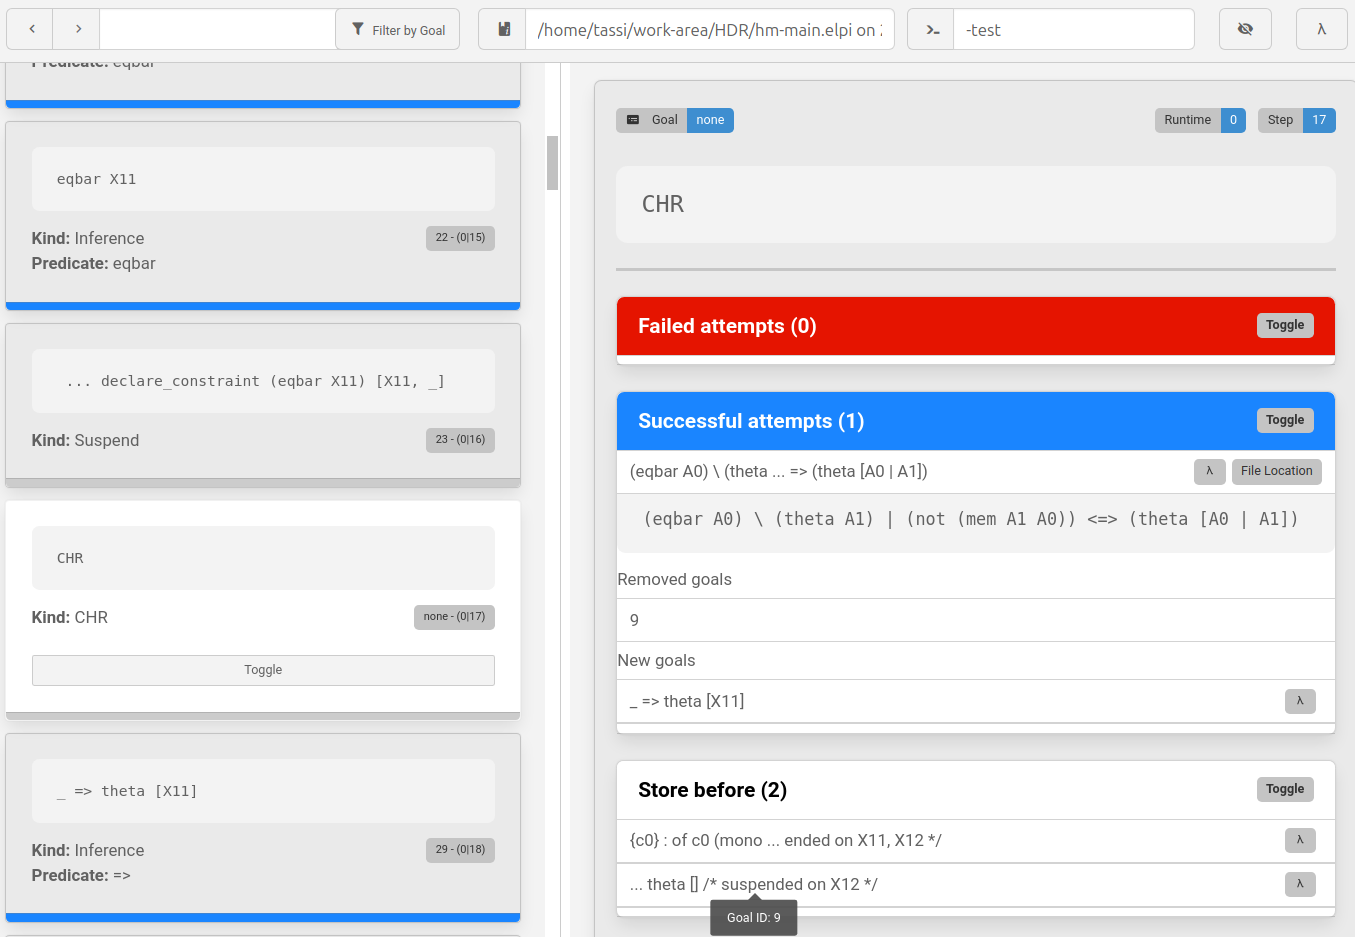
\includegraphics[width=.9\textwidth]{trace}

developed by Julien Wintz, it displays a trace as a mailbox of events
each events has pointers forward, backward and at a distance.
Each goal displays it full success or failure letting one
peek. The trace is searchable.

\chapter{Coq-Elpi}

While Elpi is a standalone language and software project, it was designed to
play the role of an \emph{extension language} for Coq. The glue between Elpi and
Coq is called Coq-Elpi.

My definition of this role, \emph{extension language}, is largely influenced
by the Lua programming language~\cite{10.5555/1200583}. Lua is an extension
language for applications written in C and is widely used in the Opens Source
world and in the gaming industry.
Its purpose is to provide an easy way to extend the host application.
It is easy to host Lua since its FFI is well curated, and thanks to that
exposing the internals of the application to the extension language requires a
limited effort to the application developer. It is easier to program in Lua,
rather than C, because the language is higher level, e.g. is features automatic
memory management and provides dictionaries as a builtin data structure.
Finally, it is easy for a user to get started with Lua because he does not need
to set up a proper development environment, the host application is sufficient
since Lua is an interpreter.\\
Elpi tries to do the same for OCaml, and Coq is the host application of interest.

Even if I'm not a big fan of it, in academia the same role is often called
meta-programming framework. Coq's main data type, terms, are programs and Elpi
programs do manipulate Coq programs. In this sense Elpi programs live at the
meta level.

\section{Why extending Coq in OCaml is hard}

Luckily OCaml features automatic memory management, types and algebraic data.
It is much, much higher level than C. Why it is hard to extend Coq then?

The first difficulty is that the complexity of the main Coq data type, terms,
is not completely hidden by the algebraic data types provided by the programming
language. The missing features are encoded and it is hard to completely hide
it to the programer (via curated APIs). In particular Coq terms feature binders
and holes. 

Binders pose two problems of their own and interact badly with holes.
The first problem is that they are typically encoded with numbers, De Bruijn
indexes, and it is just too easy to forget to shift a term.  The second program
is that when a binder is crossed on must always remember something about it,
typically the type of the bound variable. Hence the programs have to pass around
typing contexts (aka environment). It is tempting to not do it upfront, but
then one has to be disciplined. find mantra mc bride.

Holes are missing subterms and they come with metadata, a sequent.
Since the same hole can occur non linearly a single sequent is stored on the side of terms.
Moreover since binders may be reduced away each occurrence has an explicit
substitution. So there is a state that accompanies the terms, a state to be
threaded in a functional setting. This state also gathers univ constraints.
Assignment also part of this state, see also ``evar sensitive''. This is
a reified heap, we are back at memory management, pointer dereferencing (with no
types), no gc. The only thing that is easy is backracking, since the map is
purely functional.

The second difficulty is no inherent in OCaml, but rather an artifact of the
history of Coq. The API are not curated. Exposing the API in a manual, althought
not very demanding, way is key to rationalize them.


Last setting up the dev environment. I believe that can be eased with doc, but
there is another advantage in a interpreter, that you can iterate faster. Eg
in OCaml loading code is possible, but not unloading. This is even better in
a rule based language where far from the place where a code is written one
can add a rule to mask/improve/debug a piece of code.

\section{HOAS of terms and contexts}\label{GALLINA}

Global names

\begin{elpicode}
% Global objects: inductive types, inductive constructors, definitions
kind gref type.
type const constant -> gref. % Nat.add, List.append, ...
type indt inductive -> gref. % nat, list, ...
type indc constructor -> gref. % O, S, nil, cons, ...
\end{elpicode}

Terms

\begin{elpicode}
kind term type.
type sort  sort -> term. % Prop, Type@{i}
% constants: inductive types, inductive constructors, definitions
type global gref -> term.
type pglobal gref -> univ-instance -> term.
% binders: to form functions, arities and local definitions
type fun  name -> term -> (term -> term) -> term.         % fun x : t =>
type prod name -> term -> (term -> term) -> term.         % forall x : t,
type let  name -> term -> term -> (term -> term) -> term. % let x : T := v in
% other term formers: function application, pattern matching and recursion
type app   list term -> term.                   % app [hd|args]
type match term -> term -> list term -> term.   % match t p [branch])
type fix   name -> int -> term -> (term -> term) -> term. % fix name rno ty bo
type primitive primitive-value -> term.
\end{elpicode}

Context

\begin{elpicode}
pred decl i:term, o:name, o:term. % Var Name Ty
pred def  i:term, o:name, o:term, o:term. % Var Name Ty Bo
\end{elpicode}

Hence when crossing a binder

\begin{elpicode}
cross (fun N T F) :- pi x\ decl x N T => cross (F x).
\end{elpicode}

As a result of the convention, one can call \elpiinline{coq.typecheck}
deep inside a term.

\begin{ocamlcode}
MLCode(Pred("coq.typecheck",
  CIn(term, "T",
  CInOut(B.ioargC term, "Ty",
  InOut(B.ioarg B.diagnostic, "Diagnostic",
  Full (proof_context, "typchecks a term T returning its type Ty...")))),
(fun t ety diag _ proof_context _ state ->
  let sigma = get_sigma state in
  let sigma, ty = Typing.type_of proof_context.env sigma t in
  ...
\end{ocamlcode}

\ocamlinline{t} and \ocamlinline{ety} are read back in the
\ocamlinline{proof_context.env} Coq context, that is also
passed to the type checker.

Now sigma.


\section{HOAS of holes (missing terms)}

note the invariant checked when the hole materializes

\begin{elpicode}
pred evar i:term, i:term, o:term. % Evar Ty RefinedSolution
evar (uvar as X) Ty R :- declare_constraint (evar X Ty R) [X, R].
evar X Ty R :- not(var R), !, coq.typecheck R Ty ok, X = R.
evar X Ty R :- not(var X), var R, !, coq.elaborate-skeleton X Ty R ok.
 
constraint declare-evar evar def decl {

% Override the actual context
rule \ (declare-evar Ctx RawEv Ty Ev) <=> (Ctx => evar RawEv Ty Ev).
   
}
\end{elpicode}

note the chr rule allows one to set the canonical context of the evar

there is a link from Coq to Elpi

\begin{ocamlcode}
module FlexibleData : sig
  module Elpi : sig type t ... end
  module type Host = sig type t ... end
  module Map : functor(Host : Host) -> sig
    type t
    val empty : t
    val add : Elpi.t -> Host.t -> t -> t
    val elpi   : Host.t -> t -> Elpi.t
    val host : Elpi.t -> t -> Host.t
\end{ocamlcode}

%%%%%%%%%%%%%%%%%%%%%%%%%%%%%%%%%%%%%%%%%%%%%%%%%%%%%%%%%%%%%%%%%%%%%%%%%%%%%%%
%%%%%%%%%%%%%%%%%%%%%%%%%%%%%%%%%%%%%%%%%%%%%%%%%%%%%%%%%%%%%%%%%%%%%%%%%%%%%%%
%%%%%%%%%%%%%%%%%%%%%%%%%%%%%%%%%%%%%%%%%%%%%%%%%%%%%%%%%%%%%%%%%%%%%%%%%%%%%%


\section{Vernacular language integration}

While the language of Coq terms, gallina, is central to Coq-Elpi, there is another
language we have to describe first, the vernacular. That ``outern'' language
lets one organize the formalized knowledge, in particular give names to terms
and attach to them meta data.

Coq-Elpi extends the vernacular language with a few commands to declare, run
and modify Elpi programs.



\begin{figure}
\begin{coqcode}
Elpi Command hello.
Elpi Accumulate lp:{{
  main [str X] :- coq.say "Hello" X.
}}.
Elpi hello "reader".

Fail Elpi hello 46.

Elpi Accumulate lp:{{
  main [int X] :- coq.say "Hello" X.
}}.

Elpi hello 46.
\end{coqcode}
\caption[Vernacular]{Vernacular\label{vernac}}
\end{figure}

\subsection{Database, homoiconicity and rules}\label{sec:homo}

share data between programs, and programmatically add data.

maybe later?

one feature that may not look evident is that
this is allowed (unlike in teyjus)
\begin{elpicode}
build C, C => more
\end{elpicode}

and that one can actually write build

\begin{elpicode}
build F H 0 (p F :- H).
build F H N (pi x \ C x) :-
  pi x\ 
    M is N - 1,
    build (app F x) M (p x,H) (C x).
\end{elpicode}


\section{Example: simple proof transfer}\label{sec:tb}

We provide an example of a tactic and a command that communicate via
a database. The tactic \coqinline{to_bool} transfers a goal from the realm
of propositions to the one of computable (boolean) tests (decidable propositions).
The command \coqinline{register_decision} takes a proof of equivalence
between a proposition and a boolean test and ``compiles'' it to an Elpi rule.
The database contains all the known rules for translating propositions into
tests: it is queried by \coqinline{to_bool} and populated by \coqinline{register_decision}.

It is customary to organize Coq-Elpi code in this very way. The key feature
one obtains is that the \coqinline{to_bool} is extensible: when a new
predicate is declared and a new test defined, it is sufficient to call
\coqinline{register_decision} to extend \coqinline{to_bool} with the new
predicate.

We assume a Coq environment with the following lemmas. The \coqinline{reflect}
predicate links a proposition with a boolean test: \coqinline{reflect P b}
means \coqinline{P} holds if and only if \coqinline{b = true}.

\begin{coqcode}
Lemma evenP n : reflect (is_even n) (even n).

Lemma andP  {P Q : Prop} {p q : bool} :
  reflect P p -> reflect Q q -> reflect (P /\ Q) (p && q).

Lemma elimT {P b} :
  reflect P b -> b = true -> P.
\end{coqcode}

The database holds rules for the \elpiinline{tb} relation. Since
we are only interested in one direction of the equivalence we
relate a proposition with its equivalence proof (disregarding the
associated boolean test).

\begin{coqcode}
Elpi Db tb.db lp:{{

% [tb P R] finds [R : reflect P b] for some b
pred tb i:term, o:term.

:name "tb:fail"
tb Ty _ :- coq.error "Cannot solve" {coq.term->string Ty}.

}}.
\end{coqcode}

The database only contains one rule aborting the search with an error message.
All rules will need to be placed before that one.

The \coqinline{to_bool} tactic is built as follows a top of the
database.

\begin{coqcode}
Elpi Tactic to_bool.
Elpi Accumulate Db tb.db.
Elpi Accumulate lp:{{

solve (goal Ctx _ Ty _ _ as G) [G1] :-
  tb Ty P,
  refine {{ elimT lp:P _ }} G [G1].

}}.
\end{coqcode}

The tactic simply queries the database for a proof \elpiinline{P} that
the goal is related to a boolean test, then refines the goal (as in the
standard Coq \coqinline{refine} tactic) with \coqinline{elimT lp:P _}.
The hole stands for the proof of \coqinline{b = true}, i.e. the subgoal
\elpiinline{G1}.

The most interesting part of this example is how the dabase is populated.
We shall write a \elpiinline{compile} procedute that given \coqinline{evenP}
and \coqinline{andP} synthesizes the following Elpi code

\begin{elpicode}
tb {{ is_even lp:N }} {{ evenP lp:N }} :- !.
tb {{ lp:P /\ lp:Q }} {{ andP lp:PP lp:QQ }} :- !, tb P PP, tb Q QQ.
\end{elpicode}

As sketched in~\ref{sec:homo}, the two rules above corrspond to the
following (closed) Elpi terms:

\begin{elpicode}
pi N\ tb {{ is_even lp:N }} {{ evenP lp:N }} :- [!]
pi P Q PP QQ\ tb {{ lp:P /\ lp:Q }} {{ andP lp:PP lp:QQ }} :-
  [!, tb P PP, tb Q QQ].
\end{elpicode}

It is worth unfolding quotations to see that a few more quantifications are
necessary for the second rule

\begin{elpicode}
pi P Q p q PP QQ\
  tb (app[global (indt "/\"), P, Q])
     (app[global (con "andP"), P, Q, p, q, PP, QQ]) :-
  [!, tb P PP, tb Q QQ].
\end{elpicode}
  

Now that all quantifications are explicit we can look at the types of
\coqinline{evenP} and \coqinline{andP} and remark how each \elpiinline{pi}
Elpi quantification corresponds to a Coq quantification (dependent or not),
and Coq premises corresponds to recursive calls in Elpi.

\begin{coqcode}
evenP : ∀n, reflect (is_even n) (even N).
andP : ∀P Q p q,
  reflect P p -> reflect Q q -> reflect (P /\ Q) (p && q).
\end{coqcode}

The \elpiinline{compile} predicate has three inputs an one output.
The first input is the type of a lemma and the second is the proof of that
lemma, this relation between the first two argument is a key invariant.
The third argument is a list of recursive calls, while the output is
the code of the Elpi rule being generated.

\begin{elpicode}
pred compile i:term, i:term, i:list prop, o:prop.

compile {{ reflect lp:Ty _ }} P Hyps (tb Ty P :- [! | Hyps]).

compile {{ reflect lp:S _ -> lp:T }} P Hyps (pi h\ C h) :- !,
  pi h\ compile T {{ lp:P lp:h }} [tb S h | Hyps] (C h).

compile {{ ∀x, lp:(T x) }} P Hyps (pi h\ C h) :-
  pi x\ compile (T x) {{ lp:P lp:x }} Hyps (C x).
\end{elpicode}

The first rule is the base case. When we reach the conclusion of the lemma
\coqinline{reflect lp:Ty _} we know that the second argument \elpiinline{P}
is a proof of that fact, hence \elpiinline{tb Ty P} is a correct head for the
rule. The premises of the rules are the \elpiinline{Hyps} recursive calls
prefixed with a cut.

The second rule is for premises that are turned into recursive calls. In this
case the output rule features an extra \elpiinline{pi} quantification and the
\elpiinline{Hyps} list gets longer. The \elpiinline{h} variable stands for
the proof obtained by the recursive call, a proof of \coqinline{reflect lp:S _}
hene an argument we can pass to the second argument as in \coqinline{lp:P lp:h}
so to keep the invariant that it is a proof of \elpiinline{T}, the type
in which we recurse.

The last rule is a simpler version of the second, in this case the quantification
is not a premise, hence we do not extend \elpiinline{Hyps}.

The code of the \coqinline{register_decision} command located the
given lemma, finds its type and generates the new rule \elpiinline{C}.
finally it adds the rule to the database before the \elpiinline{"tb:fail"}
anchor point.

\begin{coqcode}
Elpi Command register_decision.
Elpi Accumulate Db tb.db.
Elpi Accumulate lp:{{
    
main [str S] :-
  coq.locate S GR,
  coq.env.typeof GR Ty,
  compile Ty (global GR) [] C,
  coq.elpi.accumulate _ "tb.db" (clause _ (before "tb:fail") C).

}}.
\end{coqcode}

We can now populate the database and test our tactic.

\begin{coqcode}
Elpi register_decision andP.

Lemma test : is_even 6 /\ is_even 4.
Proof.
elpi to_bool. (* Error: Cannot solve is_even 6 *)
Abort.

Elpi register_decision evenP.

Lemma test : is_even 6 /\ is_even 4.
Proof.
elpi to_bool. (* even 6 && even 4 = true *)
simpl.        (* true = true *)
trivial.
Qed.
\end{coqcode}
  
The Coq snippet calls the \coqinline{to_bool} tactic in a scenario
where a predicate is not (yet) registered obtaining an explicative
error message. Then it register a test for the missing predicate
and succesfully solves the goal.


\chapter{Coq applications}

In this chapter we survey the some applications developed on top of Coq-Elpi.
We put forward Derive and Hierarchy Builder, to which we contributed personally.
Last we quickly survey other applications developed by our colleagues.

\section{Derive}

The derive application is a framework to automatic
code generation, typically in response to the declaration of a new inductive
data type.

Coq itself is known to generate induction principles and equality tests.
Unfortunately it is also known to generate bad induction principles when
containers (e.g. lists) are involved and often fail to generate useful
equality tests.

I saw the opportunity to improve on that starting with the L3 internship of
Luc Chabassier that wrote the first prototype in the summer of 2017.
He succeeded in generating
equality tests and their proofs in two months. While most of the credit goes to
his learning skills, the experience confirmed that Coq-Elpi was able to support
research in this domain. Indeed the solution implemented by Luc, although
correct, was not very satisfactory since it was not modular. Improving
on that lead to~\cite{tassi:hal-01897468} that describes a skema to
generate so called deep induction principles and uses them to prove
equality tests correct. Before discussing that work I need to introduce
the swiss army knife of boilerplate code generation: parametricity.

\subsection{Parametricity}

The so called parametricy translation \cite{keller_et_al:LIPIcs.CSL.2012.381}
is a family of procedures $[\cdot]_i$ indexed by an arity $i$. We focus on the
unary one, i.e. $i=1$, and we write $U$ for any Coq universe, i.e. \coqinline{Prop}.
Given \emph{any} Coq term $t : r$, the unary parametricity
translation gives both a unary predicate $R$ on $r$, e.g. $[r]_1 = R : r \to U$
and a proof $T$ that $R$ holds for $t$, i.e. $[t]_1 = T : R~ t$ or somewhat more
confusingly if $t : r$ then $[t]_1 : [r]_1~ t$.

For example the unary parametricity translation of
\coqinline{nat} is \coqinline{is_nat : nat → U} and
the translation of \coqinline{3 : nat} is a proof that \coqinline{is_nat 3}.

\begin{coqcode}
Inductive is_nat : nat -> U :=
| is_zero : is_nat 0
| is_succ n : is_nat n -> is_nat (S n).

Definition is_nat_3 : is_nat 3 :=
  is_succ 2 (is_succ 1 (is_succ 0 is_zero)).
\end{coqcode}

One can see \elpiinline{is_nat} as a first class description of the
typing assignment, i.e. each term is equipped with a proof that
is has the expected type, i.e. \coqinline{0} with \coqinline{is_zero};
\coqinline{1} with \coqinline{is_succ 0 is_zero}, and so on.

The translation becomes interesting when the type has parameters such as
\coqinline{A} in \coqinline{list A}. In that case the translation builds
a predicate parametric in \coqinline{A} and in its translation. For example
the translation of \coqinline{list A} is a predicate
\coqinline{is_list : ∀A, (A → U) → (list A → U)},
and the translation of the constructors \coqinline{nil} and \coqinline{cons}
are:
\begin{coqcode}
is_nil: ∀A (isA : A → U), is_list A isA nil
is_cons: ∀A (isA : A → U), ∀a, isA a → 
  ∀l, is_list A isA l → is_list A isA (a :: l).
\end{coqcode}

As for the translation of natural numbers, each term comes with a proof
that is has the expected type. When the term is of type \coqinline{A},
the type parameter of the container, then it comes with a proof of \coqinline{isA},
the predicate parameter associated with \coqinline{A}.
The unary parametricity translation is the key to express, in a
systematic way, that a property holds deep inside a container.

The parametricity translation is a meta program in Coq, it cannot be implemented in
Gallina itself hence one needs a meta language to implement it.
Cyril Cohen implemented the binary parametricity translaton in the fall of 2017,
as he was interested in employing the translation in the Coq-EAL project.
We based the unary version on his code. Each translation is about 250 lines
of Elpi code.

\subsection{Deep induction}

We say that an induction principle is deep if the induction hypothesis is
available for sub terms that occur deep inside the immediate sub terms.
As an example we can take the data type of rose trees.

\begin{coqcode}
Inductive rtree A : U :=
| Leaf (a : A)
| Node (l : list (rtree A)).
\end{coqcode}

The induction principle generated by Coq is shallow: \coqinline{P} is
only available on the immediate subterms of type \coqinline{rtree}, that
in this case are none.

\begin{coqcode}
Lemma rtree_ind : ∀A (P : rtree A → U),
  (∀a : A, P (Leaf A a)) →
  (∀l : list (rtree A), P (Node A l)) →
  ∀t : rtree A, P t.
\end{coqcode}

That principle is weak since no element of \coqinline{l} in \coqinline{Node A l}
verifies \coqinline{P}. In \cite{tassi:hal-01897468} I study the synthesis
for a stronger principle where \coqinline{P} holds deep inside \coqinline{l}.

\begin{coqcode}
Lemma rtree_induction A is_A (P : rtree A → U) :
  (∀a, is_A a → P (Leaf A a)) →
  (∀l, is_list (rtree A) P l → P (Node A l)) →
     ∀t, is_rtree A is_A t → P t.
\end{coqcode}

The induction principle uses the unary parametricty
translation of \coqinline{l} and its type in order to systematically craft
the hypothesis \coqinline{is_list (rtree A) P l} that gives access to
\coqinline{P} on all elements of \coqinline{l}.

This  extra assumption comes at a price: the induction principle does not apply
to to just a tree, but to a tree \elpiinline{t} such that
\coqinline{is_rtree A is_A t} holds. This extra argument is
synthesized automatically.

For non-containers like \coqinline{nat}
we prove \coqinline{∀n, is_nat n} by induction on \coqinline{n} (no different
than how we proved \coqinline{is_nat 3} before). For containers we prove
the statement under the assumption that the predicate for the type parameter
is triviall true. E.g.

\begin{coqcode}
Lemma list_is_list A isA : (∀a, isA a) -> ∀l, is_list A isA l.
Lemma rtree_is_rtree A isA : (∀a, isA a) -> ∀l, is_rtree A isA l.
\end{coqcode}

While the assumption seems strong at first, it actually matches two relevant class
of predicates:
\begin{itemize}
  \item the one we are definig, e.g. \coqinline{nat_is_nat} fits
  \item any \coqinline{P : t -> U} we are defining by induction on the whole
    type \coqinline{t}, e.g. the \coqinline{P} of an induction principle
\end{itemize}

In order to prove the deep induction principle we need some scaffolding,
again synthesized automatically via Elpi programs. The first one
allows us to operate under a unary parametricity translation.

\begin{coqcode}
Definition is_list_functor A P Q :
  (∀a, P a → Q a) → ∀l, is_list A P l → is_list A Q l
:=
  fun (f : ∀a, P a -> Q a) =>
    fix IH l (pl : is_list A P l) {struct pl} : is_list A Q l :=
      match pl in (is_list _ _ s1) return (is_list A Q s1) with
      | is_Nil _ _ => is_Nil l pl
      | is_Cons _ _ a Pa xs Pxs =>
          is_Cons A Q a (f a Pa) xs (IH xs Pxs)
      end
\end{coqcode}

The proof is a straightforward induction on list \coqinline{l}.
We can now present the proof of the deep induction principle over rose trees:

\begin{coqcode}
Definition rtree_induction (A : U) (PA : A → U) (P : rtree A → U)
    (His_Leaf : ∀a, PA a → P (Leaf A a))
    (His_Node : ∀l, is_list (rtree A) P l → P (Node A l))
:=
  fix IH s1 (x : is_rtree A PA s1) {struct x} : P s1 :=
  match x in (is_rtree _ _ s2) return (P s2) with
  | is_Leaf _ _ a Pa =>
      His_Leaf a Pa
  | is_Node _ _ l Pl =>
      His_Node l (is_list_functor (rtree A) (is_rtree A PA) P IH l Pl)
  end.
\end{coqcode}

Remark the following type assignments:

\begin{coqcode}
l : list (rtree A)
Pl : is_list (rtree A) (is_rtree A PA) l
IH : ∀r, is_rtree A PA r -> P r
is_list_functor (rtree A) (is_rtree A PA) P IH l Pl :
  is_list (rtree A) P l
\end{coqcode}

The last term satisfies the premise of \coqinline{His_Node}, that in turn
gives the user of the induction principle access to the property \coqinline{P}
on all the elements of \coqinline{l}.

\subsection{Natural equality tests}

Now that we have a good induction principle we can prove the following
properties about the recursive program of interest.

\begin{coqcode}
Definition correct (T : Type) (eqb : T -> T -> bool) :=
  ∀x y : T, reflect (x = y) (eqb x y).

Definition correct_at (T : Type) (eqb : T -> T -> bool) (x : T) :=
  ∀y : T, reflect (x = y) (eqb x y).
\end{coqcode}

This is the form of correctness lemmas we shall prove.

\begin{coqcode}
Lemma seq_eq_correct : ∀A eqA (l : list A),
  is_list A (correct_at A eqA) l ->
    correct_at (list A) (list_eq A eqA) l
\end{coqcode}

It reads: if \coqinline{eqA} is a correct test on all elements of \coqinline{l},
then \coqinline{list_eq A eqA} is a good test for \coqinline{l}.

The interesting case the the equality test for rose trees, that reuses
the equality test for lists \coqinline{list_eq} passing the recursive call
at the \coqinline{eqA} argument.

\begin{coqcode}
Definition rtree_eq A (A_eq : A → A → bool) :=
  fix rec (t1 t2 : rtree A) {struct t1} : bool :=
    match t1, t2 with
    | Leaf a, Leaf b => A_eq a b
    | Node l, Node s => list_eq (rtree A) rec l s
    | _, _ => false
    end.
\end{coqcode}

What is remarkable is that the correctness proof for \coqinline{rtree_eq}
reuses the correctness proof for \coqinline{list_eq}.

\begin{coqcode}
Definition rtree_eq_correct (A : Type) (eqA : A -> A -> bool) :
  ∀r, is_rtree A (correct_at A eqA) r ->
        correct_at (rtree A) (rtree_eq A eqA) r
:=
  rtree_induction
    A (correct_at A eqA) (correct_at (rtree A) (rtree_eq A eqA))
    (fun (a0 : A) (Pa : correct_at A eqA a0) =>
       correct_Leaf A eqA a0 Pa)
    (fun (sib : list (rtree A))
         (Psib : is_list (rtree A)
                   (correct_at (rtree A) (rtree_eq A eqA)) sib) =>
       correct_Node A eqA sib
         (list_eq_correct (rtree A) (rtree_eq A eqA) sib Psib)).
\end{coqcode}

The proof also uses two auxiliary lemmas that are not particularly interesting,
we point the reader to~\cite{tassi:hal-01897468} for details about them.

\begin{coqcode}
correct_Node : ∀A eqA (l : list (rose A)),
  correct_at (list (rose A)) (list_eq (rose A) (rose_eq A eqA)) l ->
    correct_at (rose A) (rose_eq A eqA) (Node A l)

correct_Leaf : ∀A eqA (a : A),
  correct_at A eqA x ->
    correct_at (rose A) (rose_eq A eqA) (Leaf A x)
  \end{coqcode}
  
The final theorem can be obtained by satisfying the extra the extra
premise of the deep induction hypothesis, namely that each rose tree
is a rose tree.

\begin{coqcode}
Definition rose_eq_OK A eqA :
  correct A eqA -> correct (rtree A) (rose_eq A eqA)
:=
  fun p r =>
    rose_eq_correct A eqA
      r (rtree_is_rtree A (correct_at A eqA) p r).
\end{coqcode}

To conlude, both euqality tests and their proofs are built compositionally.
In~\cite{tassi:hal-01897468} we also discuss why these proofs can be kept opaque
without interfeering with the termination checker.

TODO Elpi instrumenta

\subsection{Fast equality tests}

The results in~\cite{tassi:hal-01897468} are futher refined in~\cite{gregoire:hal-03800154}
where we focus on the size (and hence type checking time) of the terms
synthesized. In particular the natural equality tests are quadratic: they
compare each constructor with all the others. Consequently proofs are also
quadratic in the number of constructors.

In~\cite{gregoire:hal-03800154} we devise equality tests that are pseudo
linear in size and we prove them correct in a compositional way using the deep
induction principles devised in~\cite{tassi:hal-01897468}.

We sketch here only the pseudo linear skema for rose trees. The idea
is to assign to each constructor a tag (a positive number) and
compare these tags upfront. If the tags are different then
the two rose trees are different, while if they are equal we can
uniformly unpack the fields and compare them.

We synthesize upfront these three functions.

\begin{coqcode}
Definition tag A : rtree A -> positive.
Definition fields_t : positive -> Type.
Definition fields A :  ∀r : rtree A, fields_t (tag t).
\end{coqcode}

The main code mattern matches over the first \coqinline{rtree} and 
pre-computes its tag and fields. The it calls a common piece of
code \coqinline{eqb_body} that will test if the tags agree and proceed
if it is the case.

\begin{coqcode}
Definition rose_eqb A eqA : rtree A -> rtree A -> bool := 
  fix rec (x1 x2 : rose A) {struct x1} : bool :=
    match x1 with
    | Leaf _ a =>
        (* 1 = tag (Leaf _ a); a = fields (Leaf _ a) *)
        eqb_body 1 (eqb_fields A eqA rec) a x2
    | Node _ sib =>            
        (* 2 = tag (Node _ sib); sib = fields (Node _ sib) *)
        eqb_body 2 (eqb_fields A eqA rec) sib x2
    end.
\end{coqcode}

When the tags agree, \coqinline{eqb_body} extracts the fields
of the second rose tree and calls \coqinline{eqb_fields}.
Since the two fields have, respectively, type 
\coqinline{fields_t t1} and \coqinline{fields_t t2} a cast is necessary.

\begin{coqcode}
Definition eqb_body t1 eqb_fields v1 x2 :=
  let t2 := tag x2 in
  match pos_eq_dec t2 t1 with
  | left heq =>
    let f2 : fields_t t2 := fields x2 in
    eqb_fields t1 f1 (match heq with eq_refl => f2 end)
  | right _ => false
  end.
\end{coqcode}

Comparing the fieds amounts at calling the equality test for the
right type, possibly using the recursive call to \coqinline{rose_eqb}.

\begin{coqcode}
Definition eqb_fields A eqA rec t :
  fields_t t -> fields_t t -> bool
:=
  match t as i return (fields_t i -> fields_t i -> bool) with
  | 1%positive => fun a b : A => eqA a b
  | 2%positive => fun a b : list (rtree A) =>
                    list_eqb (rtree A) rec a b
  | _ => fun _ _ => true (* impossible, only 2 constructors *)
\end{coqcode}

As we can see the two matches of the constructors are no nested, but rather
chained. Both \coqinline{rose_eqb} and \coqinline{eqb_fields} have a number
of branches proportional to the number of constructors.

The main downside is that, unless the quality tests gets extracted to
OCaml, the type cast that uses the evidence provided by \coqinline{pos_eq_dec}
has to be evaluated. The reader interested in benchmarks
can find them in~\cite{gregoire:hal-03800154}.

TODO Elpi instrumental

\section{Hierarchy Builder}

The mathmatical components library is the largest an most widely used
mathematical library for Coq. It is the pillar that was built for
tackling the mechanization of the Odd Order theorem~\cite{}.
A key ingredient of this pillar is the hierarchy of interfaces around which
the contents are orgnized and the fine tuning of the mechanisms that
link the interfaces to their instances: the elaborator of Coq is
programmed to automatically find a justification when an abstract theory
is applicable to an instance.

The Achilles'heel of the library is the barrier to entry, and while
documentation as in \cite{assia_mahboubi_2022_7118596} surely helps,
the complexity of building the hierarchy and programming the elaborator
could not be tamed by just explaining, exacly as assembly cannot be made
amenable by just documenting it. Hierarchy Builder (HB) provides a high level,
declarative language to describe the hierarchy and a ``compiler'' that
translate this language down the foundational language of Coq and takes
care of programming the elaborator to make the hierarchy work.

The design of the language was brought to our attention in Spring 2019
by Cohen Cyril, the result of fruitful discussions with other
researchers in this domain in a Dagstuhl seminar. The implementation
took six months~\cite{cohen_et_al:LIPIcs.FSCD.2020.34} and pushed
Coq-Elpi to bind a large set of Coq APIs. The ``boilerplate'' code
HB substitute with a metaprogram has to declare Coq modules, sections,
notations, implicit arguments, canonical structures \ldots in addition
to records and functions between records. HB also motivated the possibility
to pass Coq-Elpi programs arguments that are Coq declarations, such as the ones intruced by
the Reord or Definition keywords.

During the first implementation of HB, version 1.0, Elpi as a language was
really a technical advantage: its high level nature let us quickly experiment
with different solutions. Once the design was finalize, we thought that rewriting
the tool in OCaml, if necessary, would be possible. Then HB had to be substantially
changed in order to accommodate interfaces with parameters, with the objective
to reallt apply the too to the Mathematical Components library. This huge rewriting
turned out to possible since Elpi featured a type checker and that the change
could be modelled as a data type change: the description of an interface moved from
a flat list to a HOAS one, describing how bound parameters distribute over
the sub interfaces. A posteriori we think we could have done the same
refactoring to an OCaml program, but while it was natural to move to HOAS
in Elpi, it is unclear if the right reflex would have emerged in OCaml where
binding is not necessary reflected in the types.

\subsection{Mathematical Components 2.0}

Even if HB was, in principle, capable to describe all the interfaces of
the Mathematical Components library, it was still a huge effort to port the
library to HB.  We were lucky that developers and power users of
Mathematical Components agree to work on it during a week long coding
sprint~\cite{affeldt:hal-03463762}. The results surpassed our imagination:
not only the main library was ported, but many satellite projects moved to
HB as wll. Moreove, the high level language HB provided unlocked the
growth of the library, as depicted below. 

\includegraphics[width=\textwidth]{hb\_intf.png}

\includegraphics[width=\textwidth]{hb\_intfa.png}

Since the introduction of HB the number of interfaces almost doubled
after as decade long stagnancy.

During the porting TODO Elpi difficulty, perf, etc


\section{Other applications / uses}

Coq-Elpi found applications in other projects I did not participate
into directly. Here we mention the ones we are aware of.

\subsection{Algebra Tactics}

For a long time calling ring in MC was hard, one diff
being because of term
repr and cs proj. KS wrote a kit of tactics

\cite{sakaguchi:LIPIcs.ITP.2022.29}

\begin{elpicode}
ring C {{ @GRing.opp lp:U lp:In1 }} {{ @ROpp lp:R lp:OutM1 }} Out VM :-
  coq.unify-eq { rmorphism->zmod C } U ok,
  rmorphism->ring C R, !,
  ring C In1 OutM1 Out1 VM, !,
  build.opp Out1 Out.  
\end{elpicode}

key is call to unify

\subsection{Tackt and TRocq: proof transfer tool}

The need for proof transfer, Enzo Assia and later Cyril.

\cite{DBLP:conf/cpp/Blot0CPKMV23}
\cite{10.1007/978-3-031-57262-3_10}

the thesis compaares how rules can be transposed naturally.
CHR to store state, although the wekness of debugging
facilities limited its use to that, and not data manipulation.

\subsection{EIris: ???}

https://github.com/lukovdm/MasterThesisIrisElpi/blob/e7c9f2a835a523fa8937b24f06bac061e5f50ab9/latex/thesis/thesis.pdf

\subsection{BedRock's BRICK}
\subsubsection{N.E.S. -- Namespace Emulation System}

An experiment with Cyril Cohen that uses modules to emulate name spaces.
The characteristic of name spapces is that their content can esily be extended
a posteriori. In some way they mitigate the practical need to organize contents in
files and in an order that is imposed by logic.
eg in MC prime comes after lists since its natural definition uses the prime
decomposition operation that builds a list, so unless one makes a single file
of 10K lines he can't possibly put nat, div and prime in the same place.
NS allows you to do that.

The basic features of NES can be seen here

\begin{coqcode}
NES.Begin This.Is.A.Long.Namespace.
  Definition stuff := 1.
NES.End This.Is.A.Long.Namespace.

NES.Begin This.Is.A.Long.Namespace.
  Definition more_stuff := stuff. (* stuff in the namespace is visible *)
NES.End This.Is.A.Long.Namespace.

Print This.Is.A.Long.Namespace.stuff. (* = 1 *)

NES.Open This.Is.A.Long.Namespace.
Print stuff.
\end{coqcode}

\subsubsection{Derive plugins}

EqDecision, Countable, Finite, Inhabited, Lens, ToBit

\chapter{Conclusion}

\section{Summary}

In this document we presented the Elpi programming language, its implementation
and its main application as an extension language for Coq.

\subsection{Elpi the language}

The Elpi programming language stands on the shoulders of two giants, two
languages born in the '90s and extensively studied: $\lambda$Prolog and
Constraint Handling Rules. The former plays the main part as most of
Elpi programs manipulae syntax trees with binders. The latter is key to
scale the programming comfort of $\lambda$Prolog to syntax trees with holes
without tainting the language with tons of non logical, introspection, features.

In this document we stressed how the \emph{key} feature of Elpi is being rule
based. 3 points
- dynamic the language scale so well to syntax with binders
- static, makes it easy to write code that is easily extensible
- code unit, facilitates considerably self manipulation

CHALLENGE: The challenge for other simalar systems is to do~\ref{sec:tb}.

The importance of having a logic/pt foundations to draw the line between hacks.
Eg UT as inspecting two PT branches, or Gamma/gv unlike \cite[Section 8 and later]{10.1145/3236788}.

LESSON: never start from scratch

\subsection{Elpi the software}

We love to code, and coding a PL is great fun. Still the amount of
time to code a working PL would have been out of reach without an inria position
(no compulsory teaching duties) and engineering support from the institure (see
the trace browser).

ocaml good perf, imperative, gadt essential for APIs 

\subsection{Elpi the extension language for Coq}


\section{Current and future work}

If only I had a century.

\subsection{type class solver}

Fissore's PhD: HO unif, compilation, indexing

deep, helps with terms encoding, eg ...
like 2 times slower on simple code with a few rules.
optimizations for flattening list as in the app.


\subsection{static analysis}

determinacy

\subsection{Automation}

code specialization (a la mixtus)

\subsection{Tabling}

\cite{selsam2020tabledtypeclassresolution}

\subsection{Integration in Coq}

immediate uses of derive

\subsection{Runtime}

unification/runtime proved correct

\subsection{Compiler}

spilling fully studied

\subsection{Reasoning logic}

This is the part where 100 would not suffice to me, but there are smarter people out there.
Abella small step, understand input mode (renounce to the ground terms model),
understand green cut.




\nocite{*}
\printbibliography[title={Our Bibliography}, keyword=me]
\printbibliography[title={Bibliography}, keyword=they]
\end{document}